\documentclass{article}
\usepackage{graphicx} % Required for figures
\usepackage[numbers]{natbib}
\usepackage{float} % Add this in your preamble
\usepackage{amsmath}
\usepackage{amsfonts}
\usepackage[utf8]{inputenc}
\usepackage{hyperref}
\usepackage{indentfirst} % first paragraph indet

\title{paper collagen}
\author{robert.tavares}
\date{November 2023}

\begin{document}

\maketitle

\section{Introduction}

    O colágeno tipo I é uma proteína da familia dos colágenos, sendo sua classe do tipo fibrilar, ou seja, que é capaz de formar 
    fibrilas \cite{Silver2018}. Essa proteína	está presente em, praticamente, toda a matriz extracelular humana(ECM), que é 
    a base estrutural para as células e tecidos. Além disso, o colágeno tipo I pode ser encontrado na pele 
    \cite{Davison-Kotler2019-do}, tendões \cite{Tresoldi2013-qq}, tecido osseo \cite{FEDARKO201445, RicoLlanos2021}, cartilagem 
    \cite{Sophia_Fox2009-qd} e até mesmo na córnea \cite{CHEN201569}. A presença dessa proteína nas diversas estruturas do corpo 
    garante elasticidade e resistência a tração, bem como sustenção e manutenção dos tecidos \cite{Silver2018,Amirrah2022-uh}.  
    
    As moléculas de colágeno são o primeiro nivel de uma estrtura hierárquica mais complexa. Essas proteínas apresentam tamanhos
    típicos de $300$ nm de comprimento e $1,5$ nm de diâmetro, com sua forma semelhante a bastões \cite{Gelse2003,Silver2018}. 
    Naturalmente, essas moléculas podem se auto-organizar para formar fibrilas alongadas com comprimentos típicos em torno de 
    \(500 \mu m\) e diâmetro de \(500 nm\), sendo compostas por cerca de \(10^{7}\) moléculas \cite{Charvolin2019, KADLER1996, 
    Parry1984}. A forma de agregação dessas proteínas gera espaçamentos no interior dessas estruturas, esse intervalos possuem 
    um tamanho  típico de \(67 nm\) \cite{Zhu2018}. As fibrilas são blocos usados para compor as fibras de colágeno, elas possuem 
    morfologias variados dependendo de qual tecido elas irão compor \cite{Amirrah2022-uh}, contudo, seu diametro típico é em torno 
    de \(1-20 \mu m\). Essa evolução de escala do colágeno tipo I garante capacidades de transmitir e armazenar energia decorrentes
    de deformações ou movimentos dos tecidos compostos por essas proteínas \cite{Silver2008ViscoelasticityES}.

    A complexidade hierárquica das fibras de colágeno a torna um desafio para estudar sua estrutura e funções. A escala nanométrica das
    fibrilas e das proprias moléculas impõe dificuldades na investigação de suas propriedades mecânicas, exigindo equipamentos de 
    altissima precisão para tais análises \cite{Nalbach2022InstrumentFT}. Entre as técnicas empregadas, a Microscopia de Força Atômica 
    (AFM) destaca-se por sua aplicabilidade frequente no estudo detalhado das fibrilas de colágeno, com um foco particular na análise de 
    sua estrutura \cite{Andriotis2015-lx,Mull2022-br}. Pioneiramente, Van der Rijt e colaboradores \cite{Rijt} utilizaram a AFM para 
    avaliar as propriedades mecânicas de fibrilas isoladas de tendões, elucidando seu comportamento sob tensão até o ponto de falha. 
    Svensson et al desenvolveu uma tecnica usando atuador piezoelectrico e cantiléver microscópico para medir a distensão e a força 
    aplicada nas fibrilas \cite{SVENSSON2018270}, rescpectivamente. A técnica possui alta precisão nos testes de tensão até a fratura,
    mas possui um maior erro para forças baixas, comparado com a técnica de AFM \cite{ANDRIOTIS202335}.

    A literatura evidencia uma diversidade de modelos computacionais dedicados ao estudo das fibrilas de colágeno e suas características 
    mecânicas. Notavelmente, Buehler e seus colaboradores \cite{B1,B2,B3} introduziram uma metodologia baseada em granulação grossa, onde se
    trata as moléculas como particulas para fins de otimização computacional, e dinâmica molecular, que elucida profundamente a arquitetura 
    e o comportamento das fibrilas sob tensões ou em processos de degradação, e examina o efeito de componentes minerais incorporados 
    \cite{B4,Malaspina2017-qp,10.1002/jbmr.2705}. Alternativamente, uma abordagem fundamentada em primeiros princípios emprega osciladores 
    harmônicos, analogamente a molas, para simular a natureza elástica das fibrilas. Este modelo, aplicado em uma configuração bidimensional,
    foi explorado por Araújo e equipe para investigar as alterações nas propriedades mecânicas de tecidos sob influência de agentes degradativos
     \cite{Araujo}. Tal estratégia permite a aplicação de modelos de degradação na  escala microscópica no nível de fibras, na tentativa de 
    compreender efeitos da degradação de tecidos em uma escala superior, quando estes são submetidos a tensões e atividade enzimática.

    Em nosso trabalho, adotamos um modelo de Agregação Limitada por Difusão (\textit{Diffusion Limited Aggregation} - DLA) para simular 
    o processo de formação de agregados com morfologias análogas às fibrilas de colágeno \cite{Parkinson1995}. Após a formação das fibras, 
    conduzimos uma análise aprofundada de sua resistência mecânica sob a aplicação de tensões externas, empregando para tal um modelo mecânico 
    probabilístico, conforme delineado no trabalho de Parkinson et al \cite{Parkinson1997}. Essa investigação foi fundamentada em parâmetros 
    cruciais extraídos do modelo construtivo adotado. Adicionalmente, empreendemos um estudo detalhado das propriedades geométricas das fibras, 
    focando especificamente na densidade e na configuração espacial destas. Identificamos a ocorrência de avalanches durante o processo de ruptura, 
    caracterizadas por leis de escala precisas. Acreditamos que essa abordagem integrada, que combina simulação da formação com análise mecânica, possa 
    oferecer perspectivas valiosas de como as características estruturais intrínsecas das fibras contribuem para a sua funcionalidade e resistência 
    global, fornecendo insights valiosos para aplicações práticas e teóricas no campo da engenharia de materiais e ciência dos biomateriais.

\section{Metodologia}

    No presente estudo, desenvolvemos a investigação em duas etapas principais: na primeira, usamos um modelo para a formação de 
    fibrilas de colágeno para estudar sua estrutura; na segunda, analisamos as propriedades mecânicas desses agregados. 

    \subsection{Estrutura das fibrilas}

    Utilizamos um modelo baseado em Agregação Limitada por Difusão (\textit{Diffusion Limited Aggregation} - DLA) \cite{Witten1983} 
    em três dimensões para simular a formação de fibrilas de colágeno. Representamos as moléculas de colágeno como paralelepípedos 
    regulares de dimensões \(1 \times 18 \times 1\). Empregando uma rede regular cúbica, definimos o centro como a origem e fixamos 
    a primeira molécula do agregado, denominada \textit{seed}. Em seguida, novas moléculas são lançadas a partir de uma casca esférica
    de raio \(R\) e se difundem até que ocorra uma das seguintes situações: serem capturadas pelo agregado ou atingirem uma distância 
    \(2R\) em relação ao centro, caso em que a simulação é reiniciada. Esse processo está representado na Figura \ref{M1}. 

        \begin{figure}[H]
            \centering
            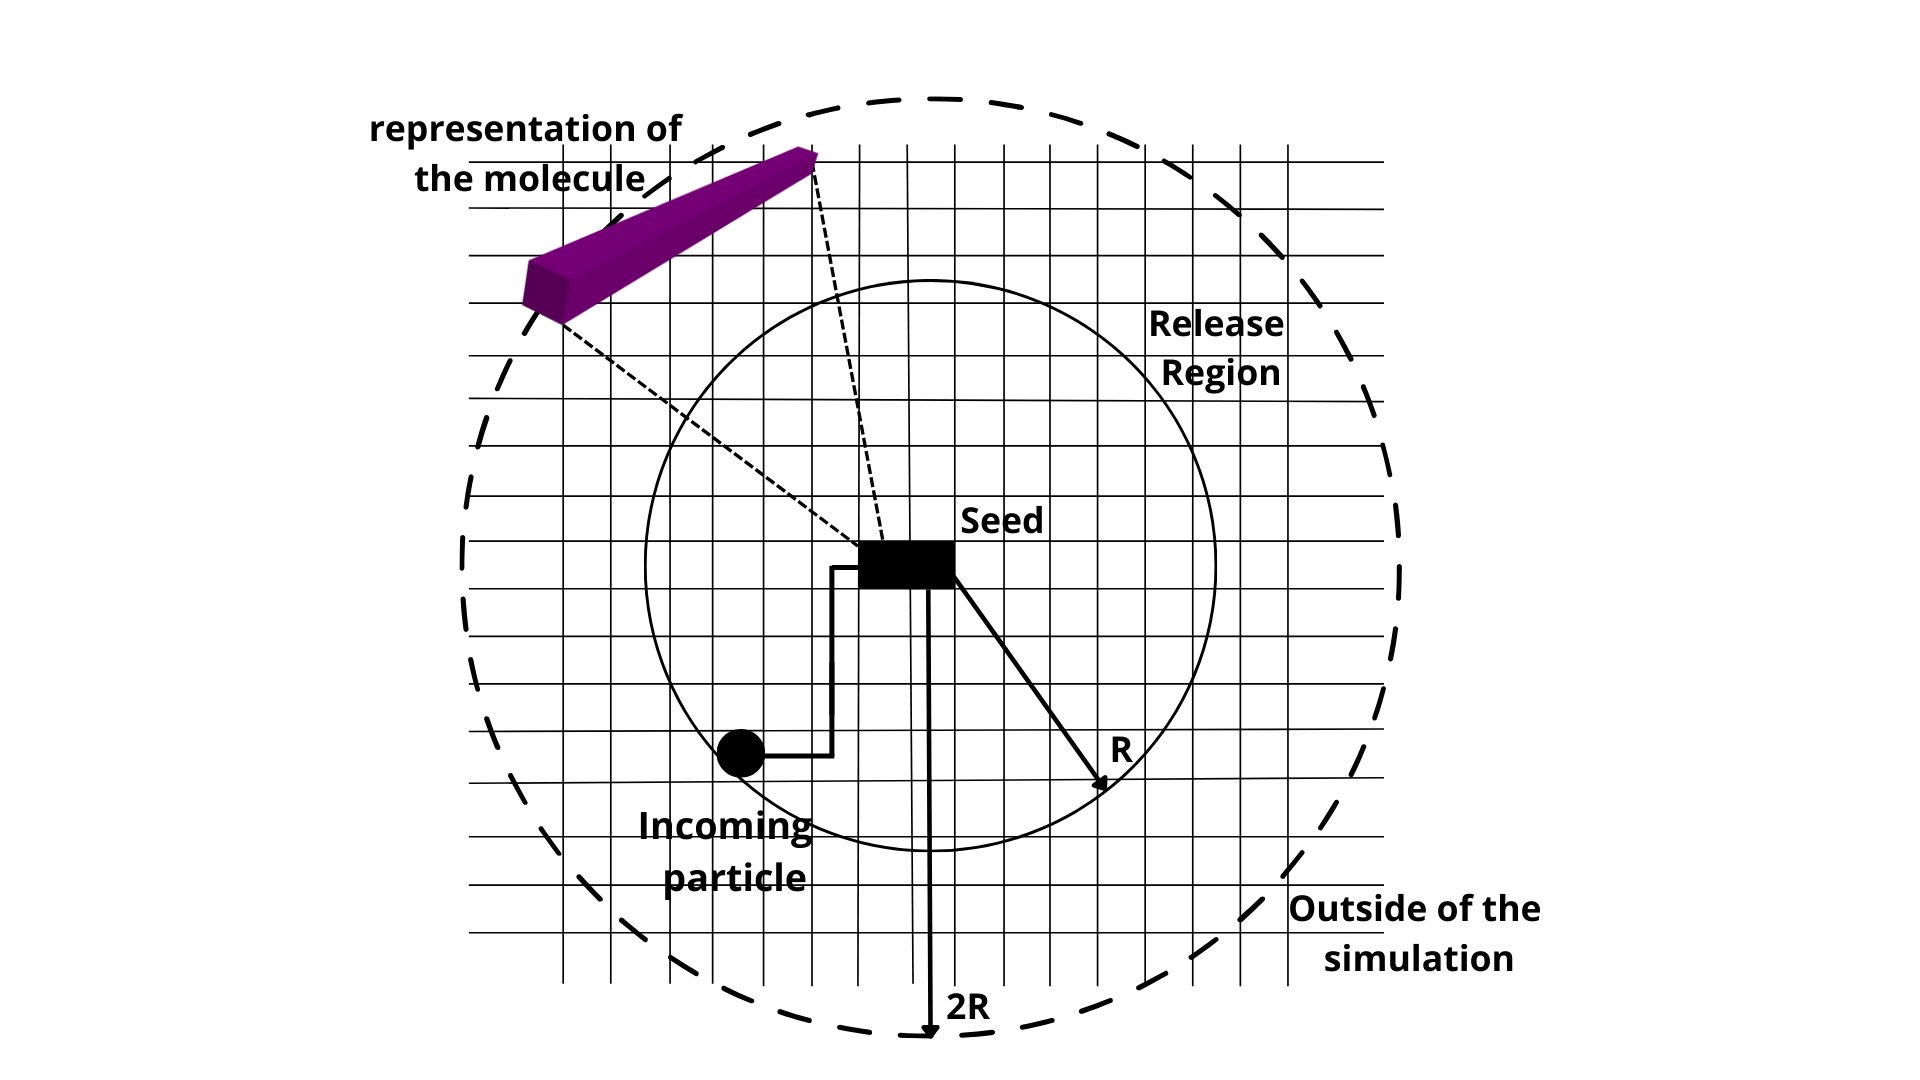
\includegraphics[width=\textwidth]{figures/DLA.png}
    
            \caption{Consideramos as moléculas de colágeno como paralelepípedos regulares de dimensões \(1 \times 18 \times 1\). 
            Estas moléculas são lançadas a partir de uma distância \(R\) da \textit{seed}, que representa a primeira molécula do
            do processo de agregação. As moléculas podem se difundir no interior de uma casca esférica até serem capturadas pelo 
            agregado ou atingirem uma distância \(2R\) da \textit{seed}, fora da zona de interesse, o que leva à reinicialização da simulação.} 
    
            \label{M1}
        \end{figure}
    
        O processo de difusão das moléculas é modelado por um \textit{random walk} tridimensional, permitindo movimentos para os primeiros e 
        segundos vizinhos no plano X-Z, enquanto no eixo Y, o movimento é restrito para frente e para trás. Na realidade, as moléculas de colágeno 
        agregam-se lateralmente e em posições escalonadas, com um comprimento característico \(D = 67 \, \text{nm}\). Assim, uma molécula é 
        capturada pelo agregado somente em posições específicas, que são múltiplos de \(D = 4\), em relação a uma molécula já pertencente ao 
        agregado \cite{Parkinson1995}. Levando em conta o tamanho representativo de 18 da nossa modelagem, identificamos cinco configurações 
        possíveis para a captura de uma molécula. A Figura \ref{M2} ilustra cada uma dessas posições possíveis, conforme descrito pela regra de 
        agregação específica. 

        \begin{figure}[H]
            \centering
            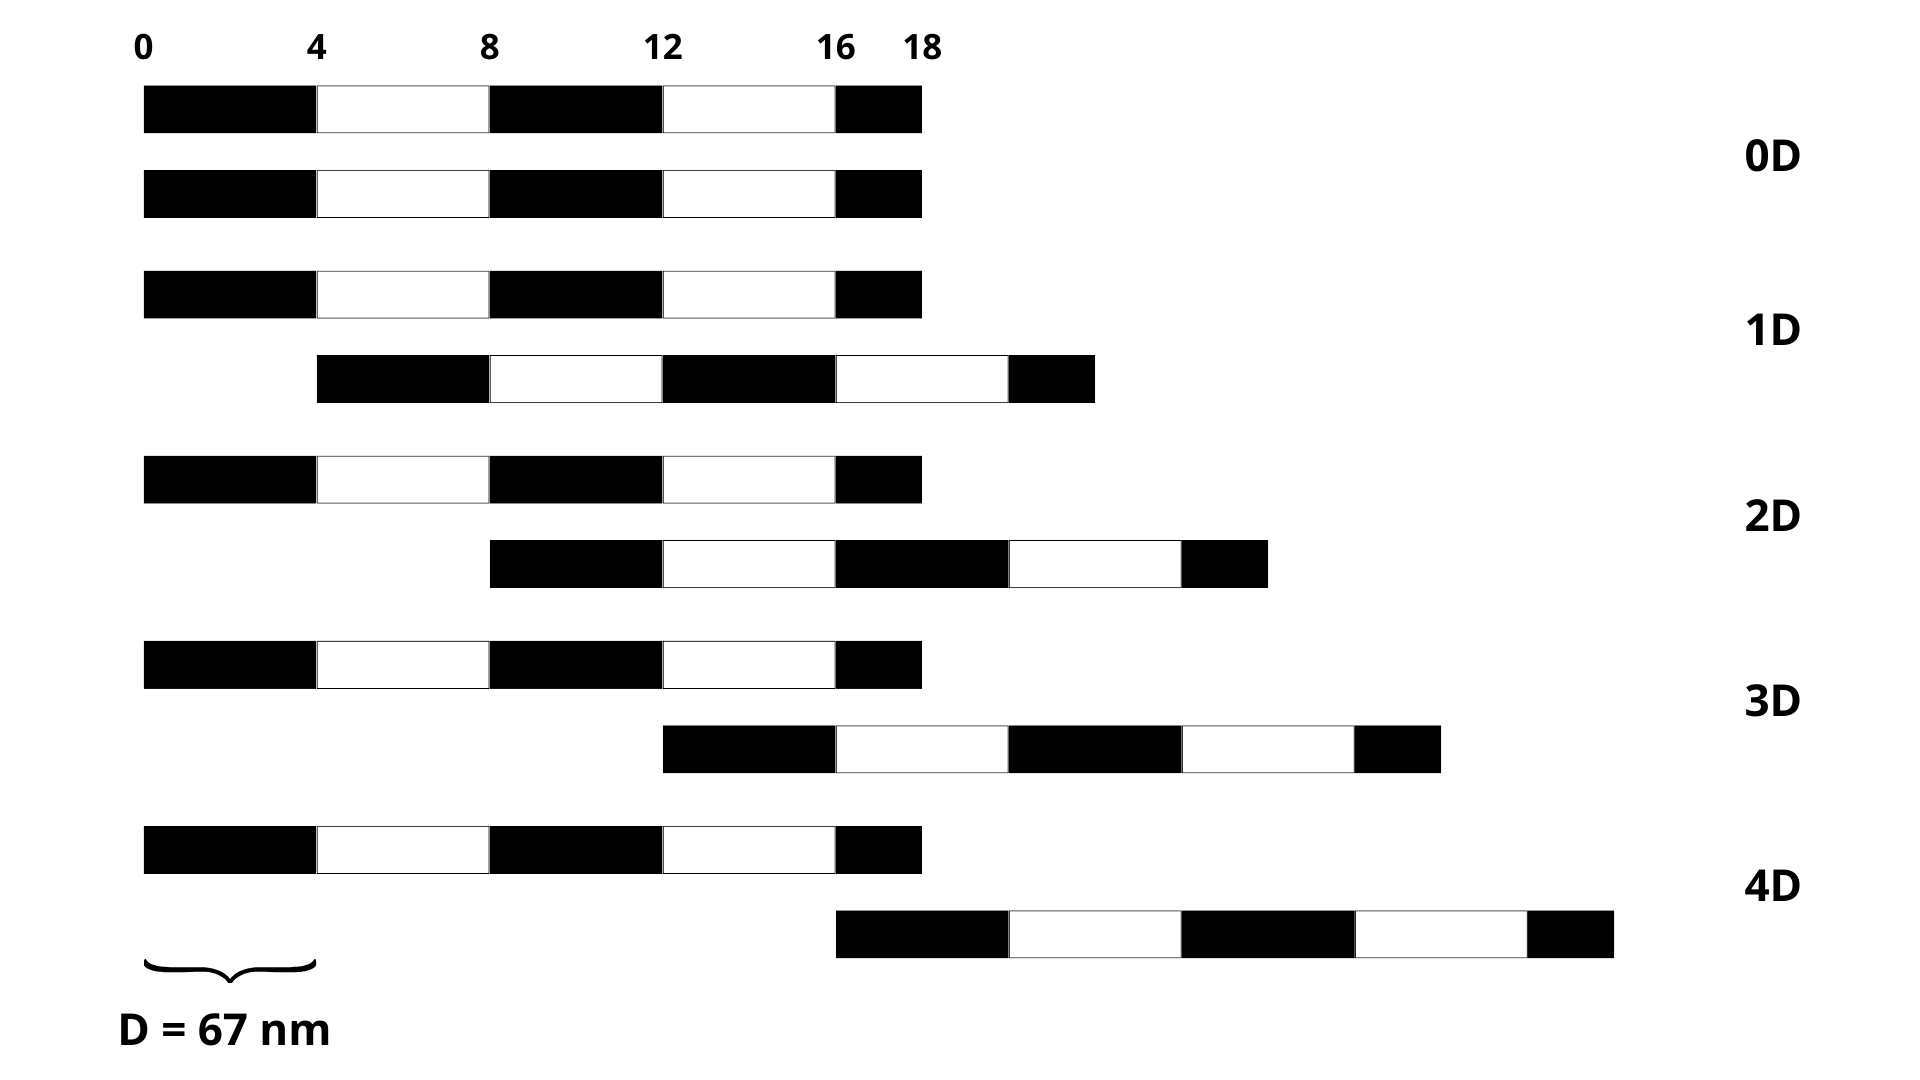
\includegraphics[width=\textwidth]{figures/specific_bind.png}
            
            \caption{Na imagem, temos uma visualização bidimensional dos objetos que representam as moléculas de colágeno na nossa simulação. 
            Esse objetos possuem um comprimento \(18\) unidades de rede e o espaçamento entre quatro unidades, representado por uma cor continua,
            equivale ao comprimento típico de \(D = 67 \, \text{nm}\) observado em moléculas reais de colágeno. Novas capturas ocorrem somente se 
            uma nova molécula estiver em contato com uma pertencente ao agregado e em uma das cinco configurações mostradas acima.}
            
    
            \label{M2}
        \end{figure}

        A formação de fibrilas reais é impulsionada por forças hidrofóbicas resultantes das interações entre as moléculas, as quais buscam 
        minimizar sua superfície exposta \cite{Kadler1987,Parkinson1995}. Implementamos um algoritmo de difusão lateral na superfície, 
        permitindo que uma molécula recém-agregada explore a superfície, mantendo sua coordenada \(y\) fixa, a fim de localizar uma posição 
        que minimize sua superfície exposta \cite{GarcaRuiz1991}. Em situações onde mais de uma posição minimiza a superfície, a  molécula 
        permanece na primeira posição encontrada. Este mecanismo é regulado pelo parâmetro \(T_{s}\), que determina o número de tentativas 
        disponíveis para a molécula explorar a superfície do agregado \cite{Parkinson1995}.

        Utilizando esse algoritmo e levando em consideração que as fibrilas variam suas características estatisticamente, optamos por gerar 
        \(50\) fibrilas, cada uma contendo \(30.000\) bastões, para diferentes valores de \(T_{s}\), a fim de investigar o efeito desse 
        parâmetro na morfologia das fibrilas. 


    \subsection{Propriedades Mecânicas} 

        \indent Para a análise das propriedades mecânicas das fibrilas, adotamos um modelo mecânico probabilístico\cite{Parkinson1997}, 
        diferente das abordagens encontradas em \cite{Saitoh2020MolecularDS} onde as fibras são represntadas por meio de um conjuntos de 
        molas acopladas.
        
        Primeiramente, realizamos o corte de um tronco de dimensão \(17 \times 201 \times 17\) em uma fibrila. Após este 
        corte, procedemos com uma limpeza para assegurar a ausência de moléculas desconectadas devido ao corte e para 
        determinar o esqueleto ativo. Consideramos que o tronco é composto por \(201\) camadas, e cada molécula, dividida 
        em parcelas de tamanho unitário, pode estender-se por mais de uma camada. Para análise das fibrilas, realizamos 
        inicialmente o corte de um tronco com dimensões 17×201×17. Procedemos com um processo de limpezanesse tronco a fim 
        de obter o esqueleto ativo, que efetivamente conduz a força na fibrila. Iniciamos pela primeira camada do tronco, 
        marcando como ativas todas as moléculas que possuem ao menos um segmento nesta camada. Em seguida, avançamos para 
        as camadas superiores e, para cada segmento ativo em uma dada camada, verificamos a existência de vizinhos ativos. 
        Caso existam, a molécula correspondente é marcada como ativa. Este procedimento é repetido até alcançarmos a última 
        camada. Com o conjunto de moléculas ativas identificado, as inativas são descartadas e o processo é então repetido, 
        agora iniciando da camada 201 e procedendo em direção à primeira camada.. Este procedimento é repetido até alcançarmos a última camada, conforme 
        ilustrado na Figura \ref{M3}. Com essa seleção de moléculas ativas, repetimos o processo agora de cima para baixo 
        até obtermos o esqueleto ativo, que é o conjunto de moléculas através do qual uma força aplicada pode percolar. 

        \begin{figure}[H]
            \centering
            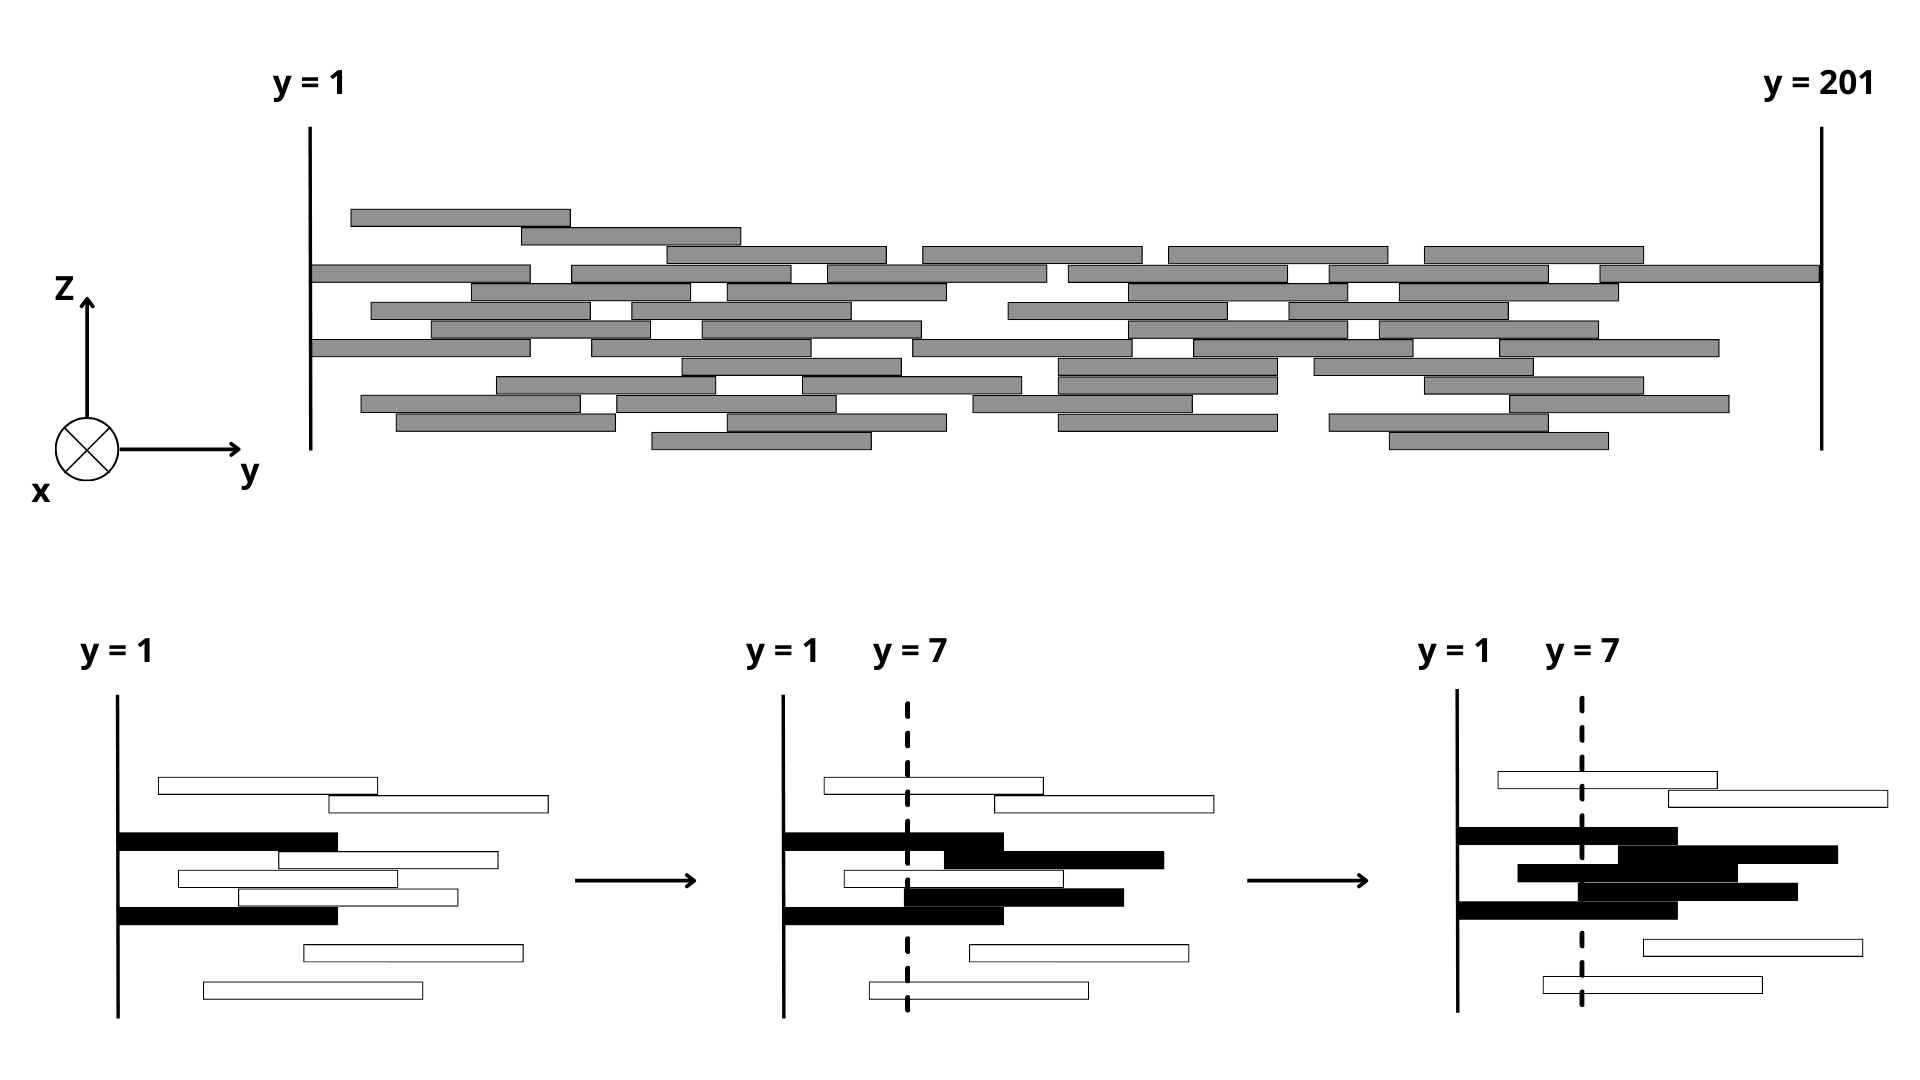
\includegraphics[width=\textwidth]{figures/esqueleto.png}
    
            \caption{Em (A) mostramos a seção selecionada para que possamos identificar o esqueleto ativo, parte da fibrila
            que efetivamente sofre a força aplicada. Em (B), da esquerda para direita ilustramos os passos nescessários 
            até identificação do agregado que definimos como esqueleto ativo. À medida que o processo evolui destacamos 
            em preto a parte ativa da fibra que efetivamente sofre a força externa aplicada. O processo ocorre até 
            atigirmos a extremidade oposta da fibra.}  
    
            \label{M3}
        \end{figure}

        Quando uma força externa é aplicada as extremidades da fibra, cada molécula que compõe a fibra sofre uma parcela 
        dessa força total, proporcional ao número de partículas presentes em sua respectiva camada. Consequentemente, em 
        uma dada \(i\)-ésima camada contendo \(M\) partículas, a equipartição da força sentida por cada molécula é aproximada
         por:  

        \begin{equation}
            \sigma_{i} \approx \frac{F}{M_{i}},
        \end{equation}
            

        \noindent onde \(\sigma_{i}\) representa a tensão sentida por cada particula na \(i\)-ésima camada e \(F\) é a força 
        total aplicada ao agregado. A força sentida por uma molécula individual no agregado é, portanto, a média dos \(\sigma_{i}\) 
        correspondentes às camadas em que a molécula está presente. 
        
        Quando temos o ropimento de uma ligação interna na estrutura essa quebra aumenta a probabilidade de outras rupturas, levando a 
        uma cascata de falhas na fibrila até acontecer um rompimento global. Dessa forma, consideramos a probabilidade de ruptura para 
        a molécula como um todo, ao invés de para cada partícula individual que a compõe. Adicionalmente, assumimos que o número de 
        ligações responsáveis por manter a molécula fixada no esqueleto ativo é igual ao somatório do número de partículas vizinhas em 
        cada camada onde a molécula está presente. 

        Com base nesses pressupostos, definimos nossa probabilidade de ruptura pela equação 

        \begin{equation}
            P_{R} = \left(\frac{\langle \sigma_{i} \rangle}{N \sigma_{s}}\right)^{m},
        \end{equation}

        \noindent onde \(N\) representa o número de ligações de uma dada molécula, \(\sigma_{s}\) denota a tensão das ligações entre as 
        moléculas, e \(m\) é um fator que modula a dissipação de energia \cite{Parkinson1997,2013}. Por questões de simplicidade, adotamos 
        \(m = 2\) em todas as nossas simulações.

        O processo de ruptura é simulado com aplicação de uma força ao esqueleto ativo, em uma tentativa de reproduzir os comportamentos observados 
        em experimentos de distensão. Inicialmente, calculamos a probabilidade de remoção \(P_{R}\) para cada molécula. Em seguida, realizamos um 
        sorteio de um valor entre 0 e 1 para cada molécula; se o valor sorteado for menor ou igual a \(P_{R}\), a molécula é removida. Este processo 
        é repetido para todas as moléculas do agregado. Após a primeira varredura, recalculamos \(P_{R}\) para as moléculas remanescentes sob a mesma 
        força aplicada e continuamos o processo até que não ocorram mais quebras. A força é então incrementada em meia unidade, e o procedimento é 
        repetido. Consideramos que a fibrila se rompe quando ao menos uma camada fica vazia, indicando que o esqueleto ativo não mais forma permitindo 
        que a força seja transmitida para a vizinhança próxima na fibra.. Esse procedimento está esquematizado na Figura \ref{M4}. Monitoramos o 
        processo de remoção das moléculas, registrando a quantidade de moléculas removidas para uma dada força e a tensão máxima suportada antes da 
        ruptura. 


        \begin{figure}[H]
            \centering
            \includegraphics[width=\textwidth]{figures/simulaçao (1).png}
    
            \caption{Na figura, em (A) representamos a fibra sujeita a uma força $F$ aplicada em suas extremidades. Cada pedaço (bloco) que compõe 
            a fibra representa um entrelaçado de moléculas que podem se romper a depender da probabilidade $P_{R}$ [Usar Eq.(2)]. Em (B) o processo 
            de ruptura é testado estatisticamente (número entre zero e um) e a depender do teste, um pedaço da fibra se rompe. Em (C), após vários 
            testes estatístico a fibra se rompe por completo na condição que há uma ruptura de uma seção transversal da fibra.} 
    
            \label{M4}
        \end{figure}

      
        Consideramos a quantidade de moléculas rompidas como um indicador da deformação da nossa fibrila. Além disso, determinamos a tensão em relação 
        às forças calculadas para aproximar a simulação a uma fibrila real. A força necessária para romper uma ligação é considerada constante, e 
        utilizamos o diâmetro médio das fibrilas para calcular a tensão. 

        Para cada valor de \(T_{s}\), selecionamos 10 fibrilas para submeter ao procedimento de simulação. Para cada fibrila, realizamos mil 
        experimentos. Registramos, para cada nível de força aplicada, o número de moléculas removidas do esqueleto e quantas permaneceram. 
        
        \subsection{Medidas de fractalidade e Tensão sobre as fibrilas}

        Para realizar a medida da fractalidade, utilizamos o tronco cortado para o teste de tensão antes da simulação ser realizada. Nos 
        realizamos uma série de cortes transversais na fibrila, indo de \(-90\) a \(90\) com \(18\) unidades de distância. Nessas seções, 
        nos utilizamos a relação massa-raio para calcular a dimensão fractal das fibrilas:

        \begin{equation}
            m \approx F_{D} \times R,
        \end{equation}

        \noindent onde \(m\) é a quantidade de particulas dentro de circulo de raio \(R\) e \(F_{D}\) a dimensão fractal.
        Nos consideramos o centro de massa da seção como o centro do disco de raio \(R\). A dimensão fractal de uma fibrila
        foi calcula como a media da dimensão sobre as seções. A dimensão fractal média de uma fibrila para dado \(T_{s}\) foi 
        calculada pela média da dimensão fractal sobre \(50\) fibrilas de mesmo parâmetro.

        Desse algoritmo, nos retiramos o raio da seção transversal como sendo o \(R\) de disco que continha todo o agregado 
        da seção. O raio medio de uma fibrila foi calculado como a média sobre o raio de cada seção para uma mesma fibrila.
        O raio médio de uma fibrila para dado \(T_{s}\) foi calculado pela média sobre \(50\) fibrilas de mesmo parâmetro.

        Como nossa fibrila, no plano X-Z, é um quadrado de lado unitário, nos consideramos que esse valor é equivalente
        ao diâmetro medio das fibrilas reais, \(500 nm\) \cite{KADLER1996, Parry1984}, desse modo, nos calculamos o raio medio
        das fibrilas em uma escala real.

        No processo de ruptura, como ele ocorre probabilísticamente, temos que a uma variação no valor de ruptura das fibrilas
        e, portanto, no tamanho dos dados, dificultando o calculo médio. Dessa forma, nos optamos pela seguinte abordagem: calculamos
        a tensão suportada média para cada fibrila para as mil simulações. Em seguida, nos consideramos apenas os dados das simulações
        que foram até o valor médio. Com isso, nos determinamos a deformação média das fibrilas. 

        Para aproximar a simulação de experimentos reais, nos consideramos que cada unidade de força usada para romper as fibrilas é
        equivalente a \( F_{c} = 0.5 nN\) \cite{Pandolfi2019AMM}, o valor calculado para ligações cruzadas em fibrilas reais. Com isso, 
        nos determinamos a tensão suportada pelas fibrilas como a razão da força pela área da seção transversal:

        \begin{equation}
            \sigma = \frac{F \times F_{c}}{\pi R^{2}},
        \end{equation}

        \noindent onde \(F\) é força que calculamos,  \( F_{c}\) o fator de conversão para a escala real e \(R\) o raio médio que determinamos
        para as fibrilas.




\section{Resultados}
    \subsection{Morfologia das fibrilas}

    Os agregados gerados pelo modelo apresentam uma morfologia fibrilar, com características relevantes quanto a sua forma 
    sendo determinadas pelo parâmetro \(T_{s}\). Podemos observar, na Figura \ref{R1}, a estrutura desses agregados 
    para os valores de \(T_{s} = 2\), baixa difusão, e \(T_{s} = 10000\), alta difusão lateral sobre a superfície. As 
    fibrilas com menor \(T_{s}\) apresentam uma forma menos densa, enquanto para valores mais altos, observamos uma 
    forma mais compacta e regular. A coloração indica o quão antiga uma molécula pertence ao agregado, indo do azul 
    escuro, mais antigas, para o amarelo, mais recentes. Nos agregados mais compactos, temos dificuldade em observar 
    moléculas mais antigas visto que essas estão localizadas no interior da estrutura. Para fibrilas menos compactas fica 
    mais fácil identificar as que pertencem ao agragado por mais tempo. Além disso, na visão lateral, observamos o 
    comportamento alongado e com pontas afinadas, típico de fibrilas reais. 

    \begin{figure}[H]
        \centering
        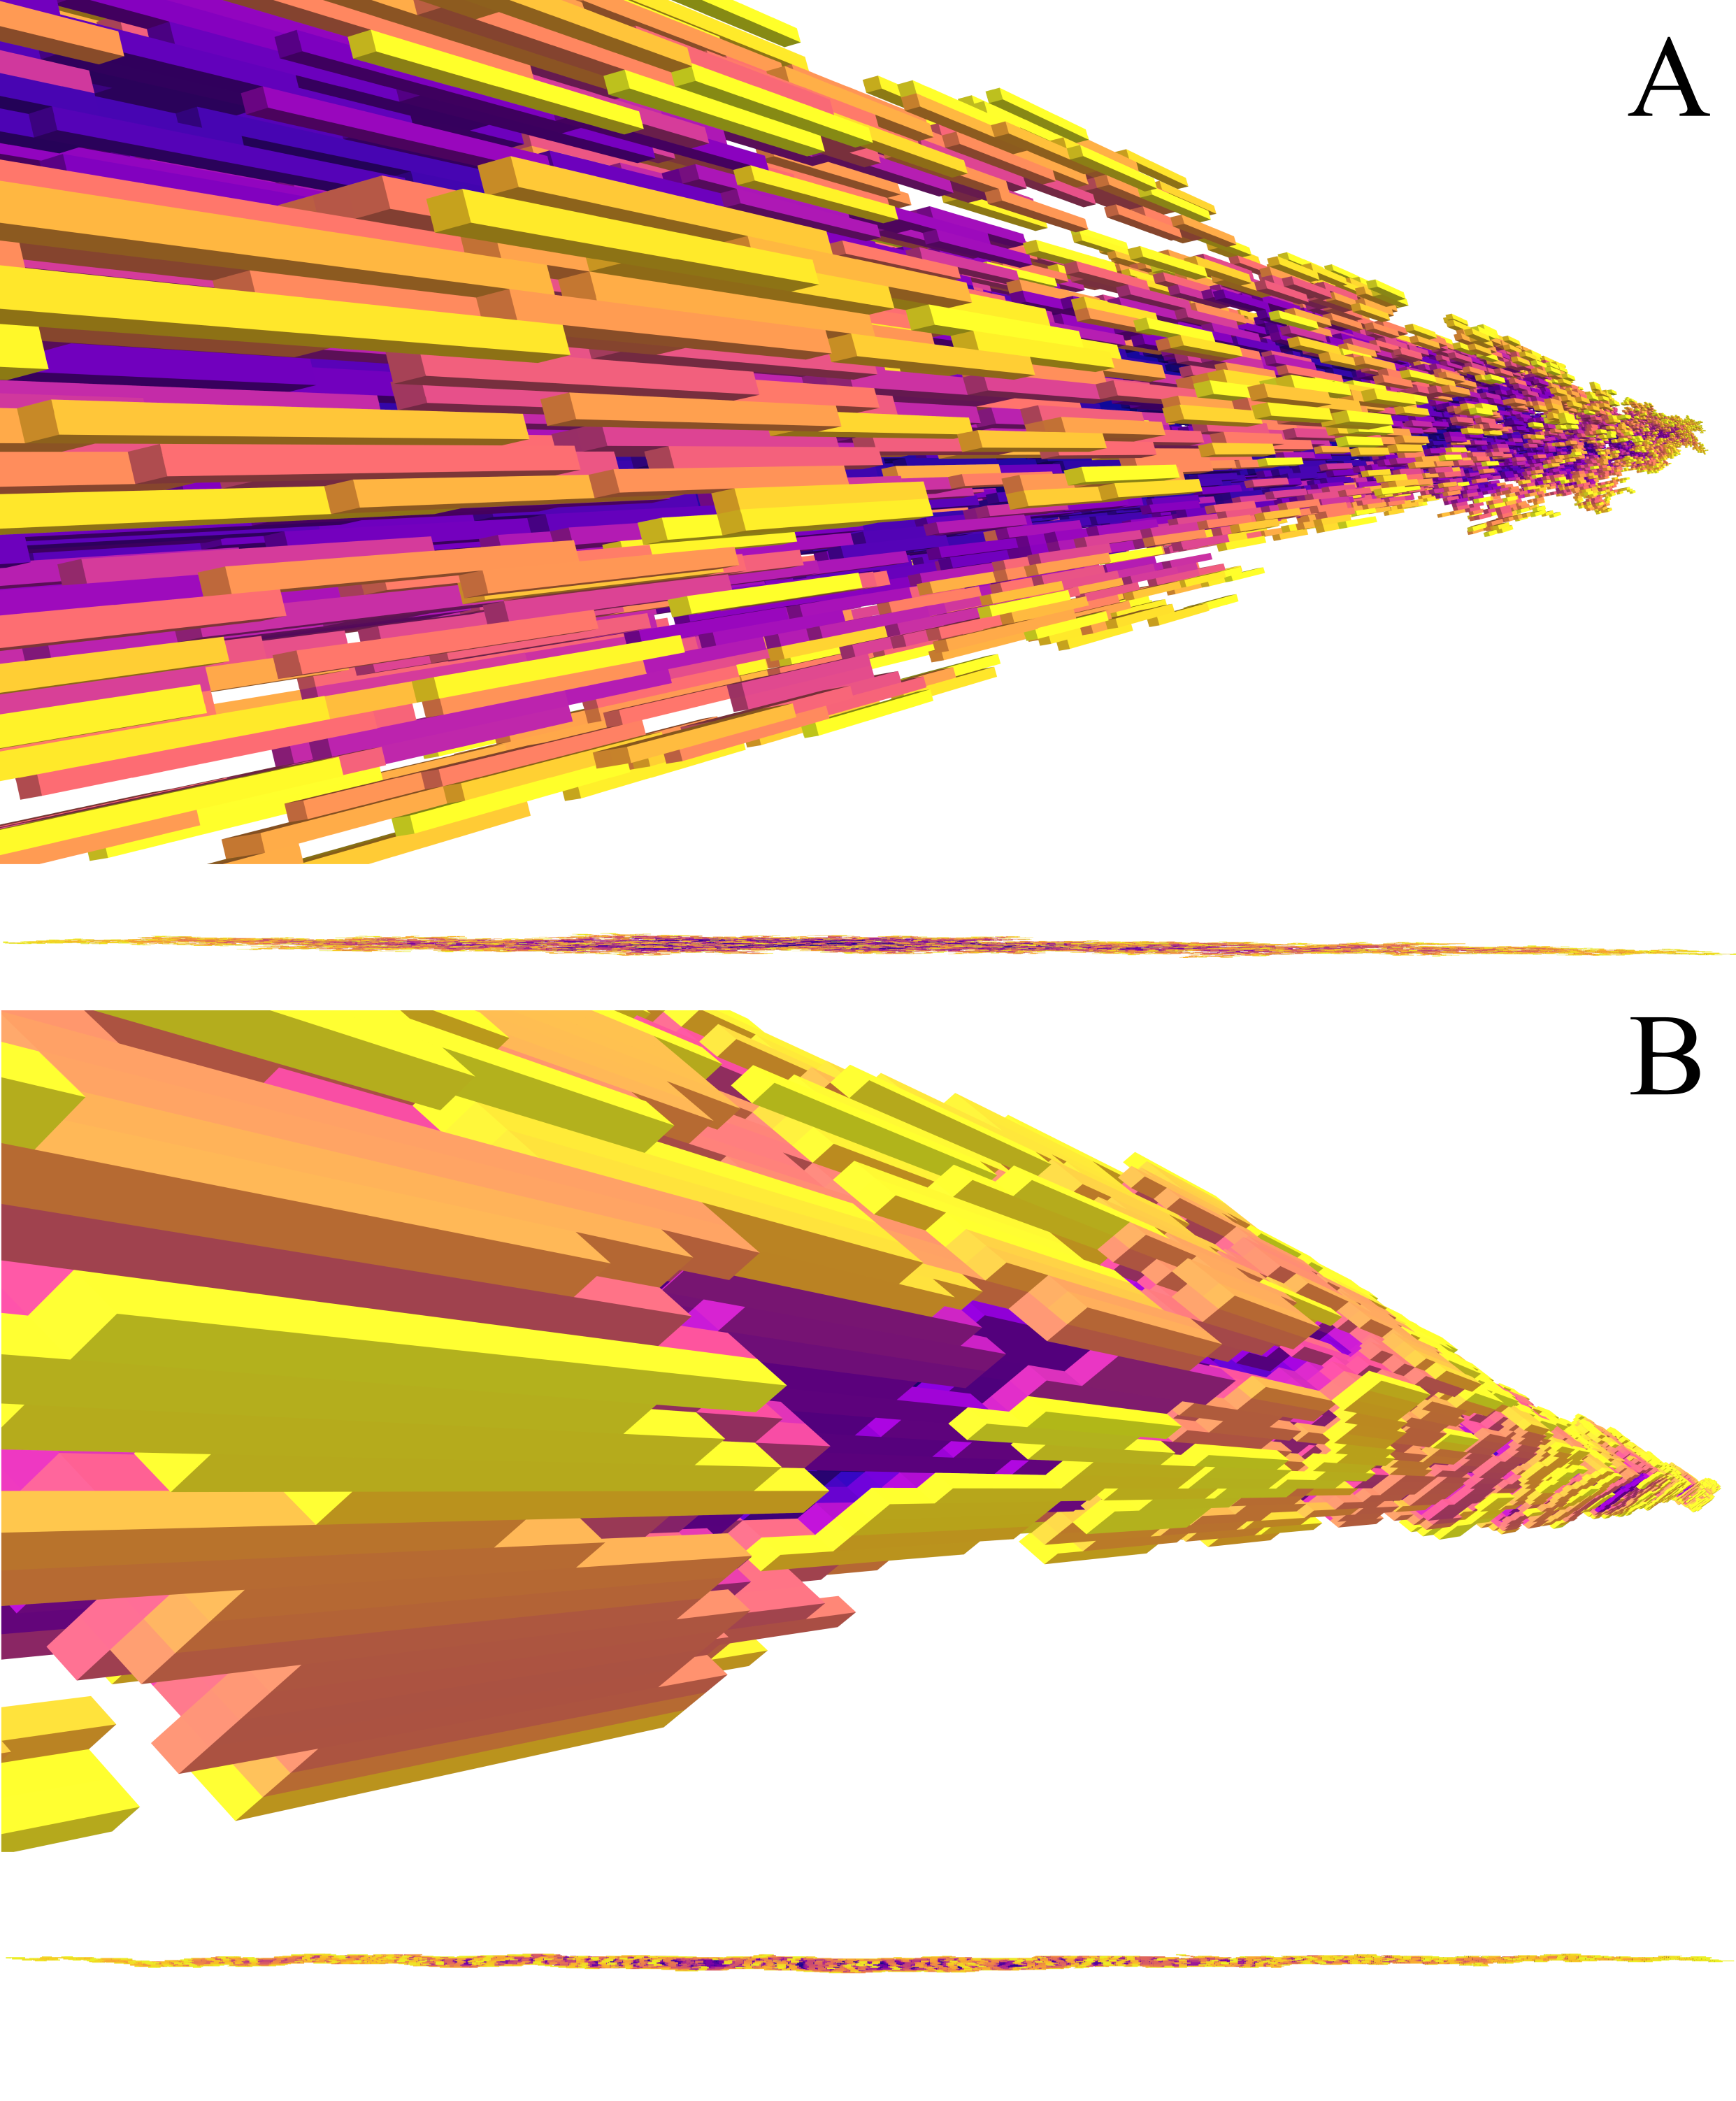
\includegraphics[width=\textwidth]{figures/fibrils.png}

        \caption{Representação das fibrilas geradas com o algoritmo de DLA contendo $30.000$ moléculas. 
        Em (A) e (B) destaque a visão transversal enquanto que abaixo uma visão lateral da região central
        das fibrilas realçando a maior compactação das fibrilas. As cores indicam 
        o tempo de pertencimento de cada bloco ao agragado. Quanto mais próximo do azul mais antigo esse 
        bloco pertence ao agregado, equanto que uma tendência para o amarelo indica um pertencimento recente 
        ao agragado. Em (A) temos uma fiblila gerada com \(T_{s} = 2\), indicando baixa difusão, enquanto que 
        em (B) temos \(T_{s} = 10000\), representando efeito de alta difusão.} 

        \label{R1}
    \end{figure}

    O comprimento, o diâmetro e a densidade(\(\rho\)) da região central das fibrilas são características influenciadas pelo 
    parâmetro \(T_{s}\). Na Tabela \ref{tab1}, podemos observar como essas dimensões se alteram, em média, com o 
    aumento desse parâmetro. Calculamos a densidade considerando o espaço ocupado pelas moléculas dentro de uma caixa
    que continha o tronco, o comportamento dessa parâmetro e do comprimento tendem a aumentar com o incremento de \(T_{s}\), enquanto 
    o diâmetro tende a diminuir. Uma propriedade comum a essas medidas é que elas exibem um comportamento de 
    estabilização à medida que nos aproximamos de \(T_{s} = 512\); a partir desse ponto, elas oscilam em torno de um 
    valor médio. 

    \begin{table}[H]
        \caption{Valores médios dos comprimentos, diametros e densidade de fibrilas geradas para diferentes valores de \(T_{s}\).}

        \centering  % Mantém a tabela centralizada no texto
        \begin{tabular}{lccc}
        \hline
        \textbf{$T_{s}$} & \multicolumn{1}{c}{\textbf{Length(u.m)}} & \textbf{Ray(u.m)} & \textbf{\(\rho\)(\%)} \\ \hline
        2                & 3668.36                                   & 32.40             & 0.17                  \\
        8                & 3695.16                                   & 28.68             & 0.25                  \\
        16               & 3764.27                                   & 24.63             & 0.34                  \\
        32               & 3808.68                                   & 21.67             & 0.46                  \\
        64               & 3891.56                                   & 17.6              & 0.57                  \\
        128              & 3928.6                                    & 16.06             & 0.62                  \\
        512              & 3913.24                                   & 14.07             & 0.66                  \\
        1024             & 3912.52                                   & 14.14             & 0.65                  \\
        4096             & 3892.28                                   & 14.06             & 0.66                  \\
        8192             & 3892.52                                   & 14.16             & 0.66                  \\
        10000            & 3917.16                                   & 13.94             & 0.65                  \\ \hline
        \multicolumn{1}{l}{Limit Upper} & 3905.54                    & 14.08             & 0.65                  \\ \hline
        \end{tabular}
        \label{tab1}  % Substitua 'meu_rótulo' pelo rótulo desejado para a referência cruzada
    \end{table}


    Outra característica desses agregados é a relação linear entre a massa e a distância até as pontas. Na Figura 
    \ref{R2}, observamos que, independentemente do valor de \(T_{s}\), todos os agregados exibem esse comportamento. 
    Tal característica é recorrentemente observada tanto em fibrilas reais quanto nas simuladas com este modelo 
    \cite{Parkinson1995,Kadler1987}. 


    \begin{figure}[H]
        \centering
        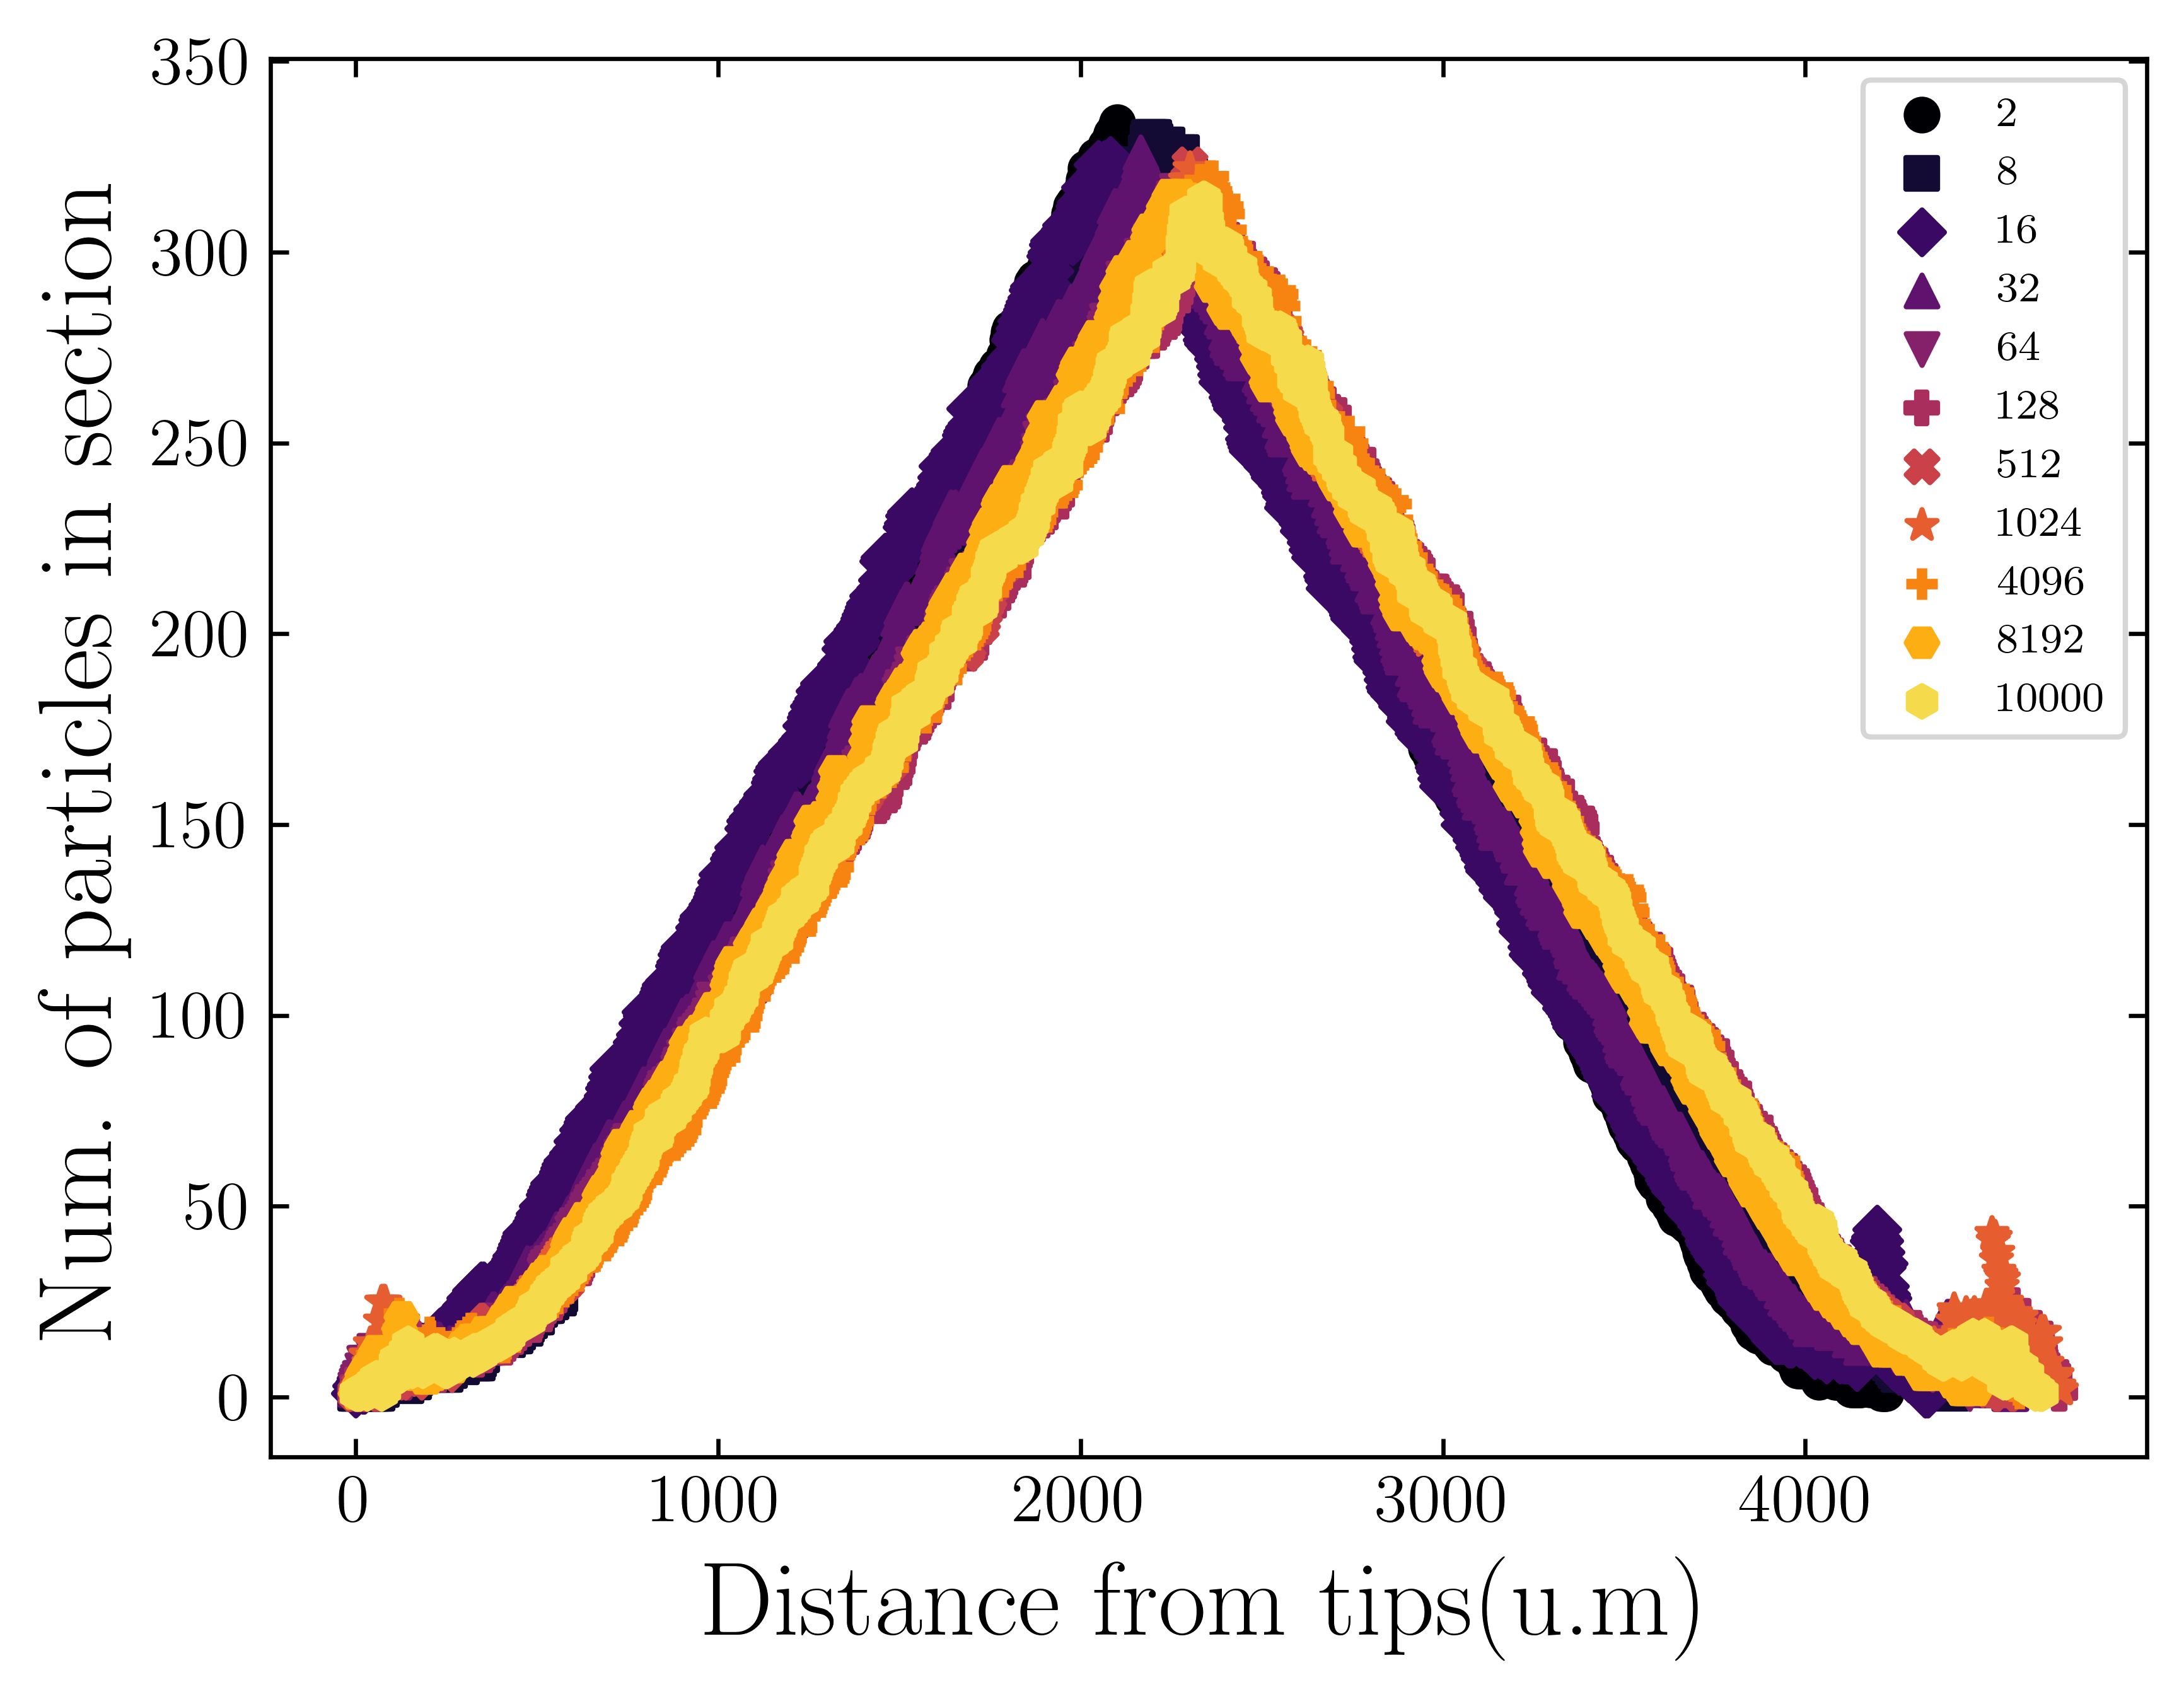
\includegraphics[width=\textwidth]{figures/tips.png}

        \caption{A figura mostra a quantidade de partículas por seção tranversal das fibrilas geradas em função da 
        distância desta seção até a sua extremidade. Partindo de uma ponta, a massa cresce linear até bem proximo 
        da região central da fibrila. A medida que nos afastamos dessa região, a massa decaí linearmente. Os simbolos 
        correspondem aos diferentes valores de $T_{S}$. Fica evidente que o valor escolhido para $T_{S}$ não tem 
        efeito sobre esse efeito.} 

        \label{R2}
    \end{figure}


    Com o objetivo de obter um entendimento mais preciso acerca do efeito do parâmetro $T_{S}$ sobre a morfologia das 
    fibrilas geradas analisamos a seção transversal na posição \(y=0\), conforme ilustrado na Figura \ref{R3}. Observamos 
    que o aumento do parâmetro \(T_{s}\) resulta na diminuição dos espaços vazios dentro da seção, levando à formação de 
    agregados mais compactos e quase completamente preenchidos. Devido a essa característica progressiva em função do 
    parâmetro \(T_{s}\) e de seu aspecto não euclidiano, optamos por calculara dimensão fractal das seções e constatamos que, à medida que \(T_{s}\) aumenta, ocorre um 
    incremento no valor médio da dimensão fractal da seção até atingir uma saturação. Na Figura \ref{R4}, é evidente 
    que para valores mais baixos de \(T_{s}\), a dimensionalidade é próxima da observada em agregados gerados pelo 
    modelo de Agregação Limitada por Difusão (DLA) \cite{Witten1983}, que é de 1.71, recuperando os valores esperados 
    que remete aos igredientes básicos presente em nosso modelo de formação. Por outro lado,, para valores mais elevados 
    de \(T_{s}\), a dimensão fractal tende a estabilizar em valores próximos a 1.93, que se assemelha muito à dimensão 
    euclidiana para objetos bidimensionais. 

    \begin{figure}[H]
        \centering
        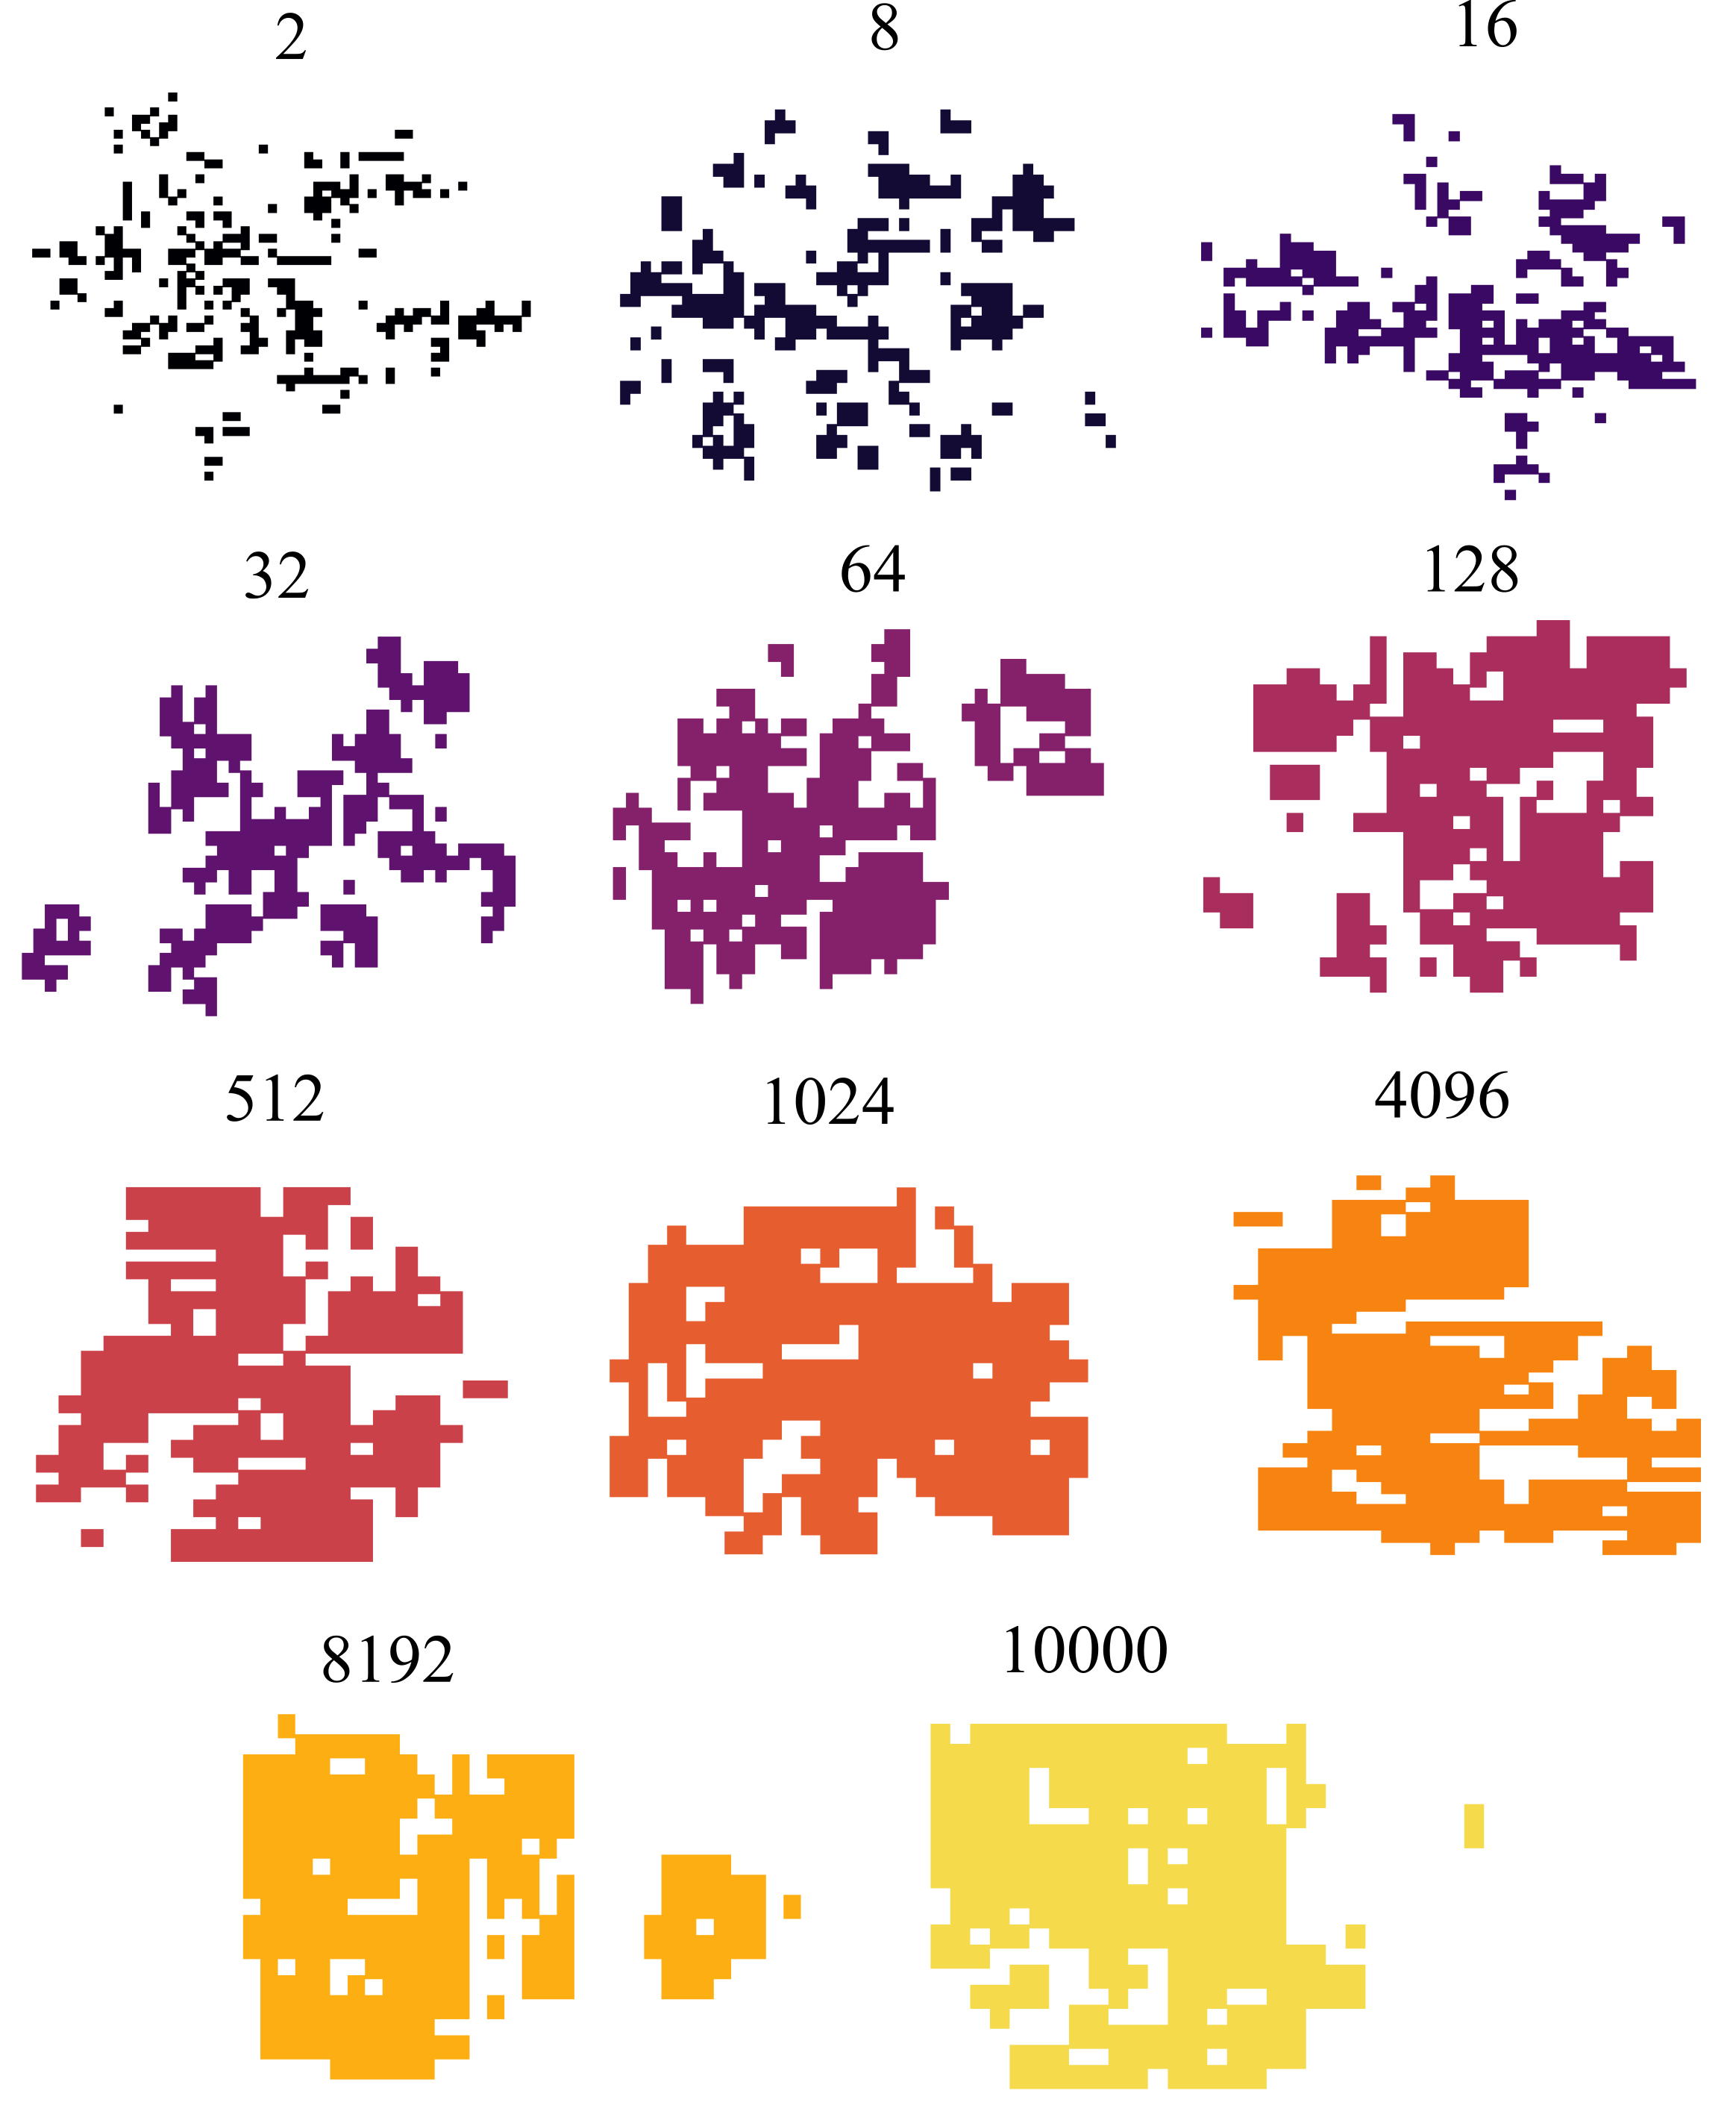
\includegraphics[width=\textwidth]{figures/cs_all.png}
        \caption{A figura mostra a visualização de diferentes cortes transversais localizados em \(y=0\) para diferentes 
        valores do parâmetro \(T_{S}\). Da esquerda para direita e de cima para baixo temos os seguintes valores para o 
        prâmetro \(T_{S}=2,8,16,32,64,128,512,1024,4096,8192, 10000\).} 
        \label{R3}
    \end{figure}

    \begin{figure}[H]
        \centering
        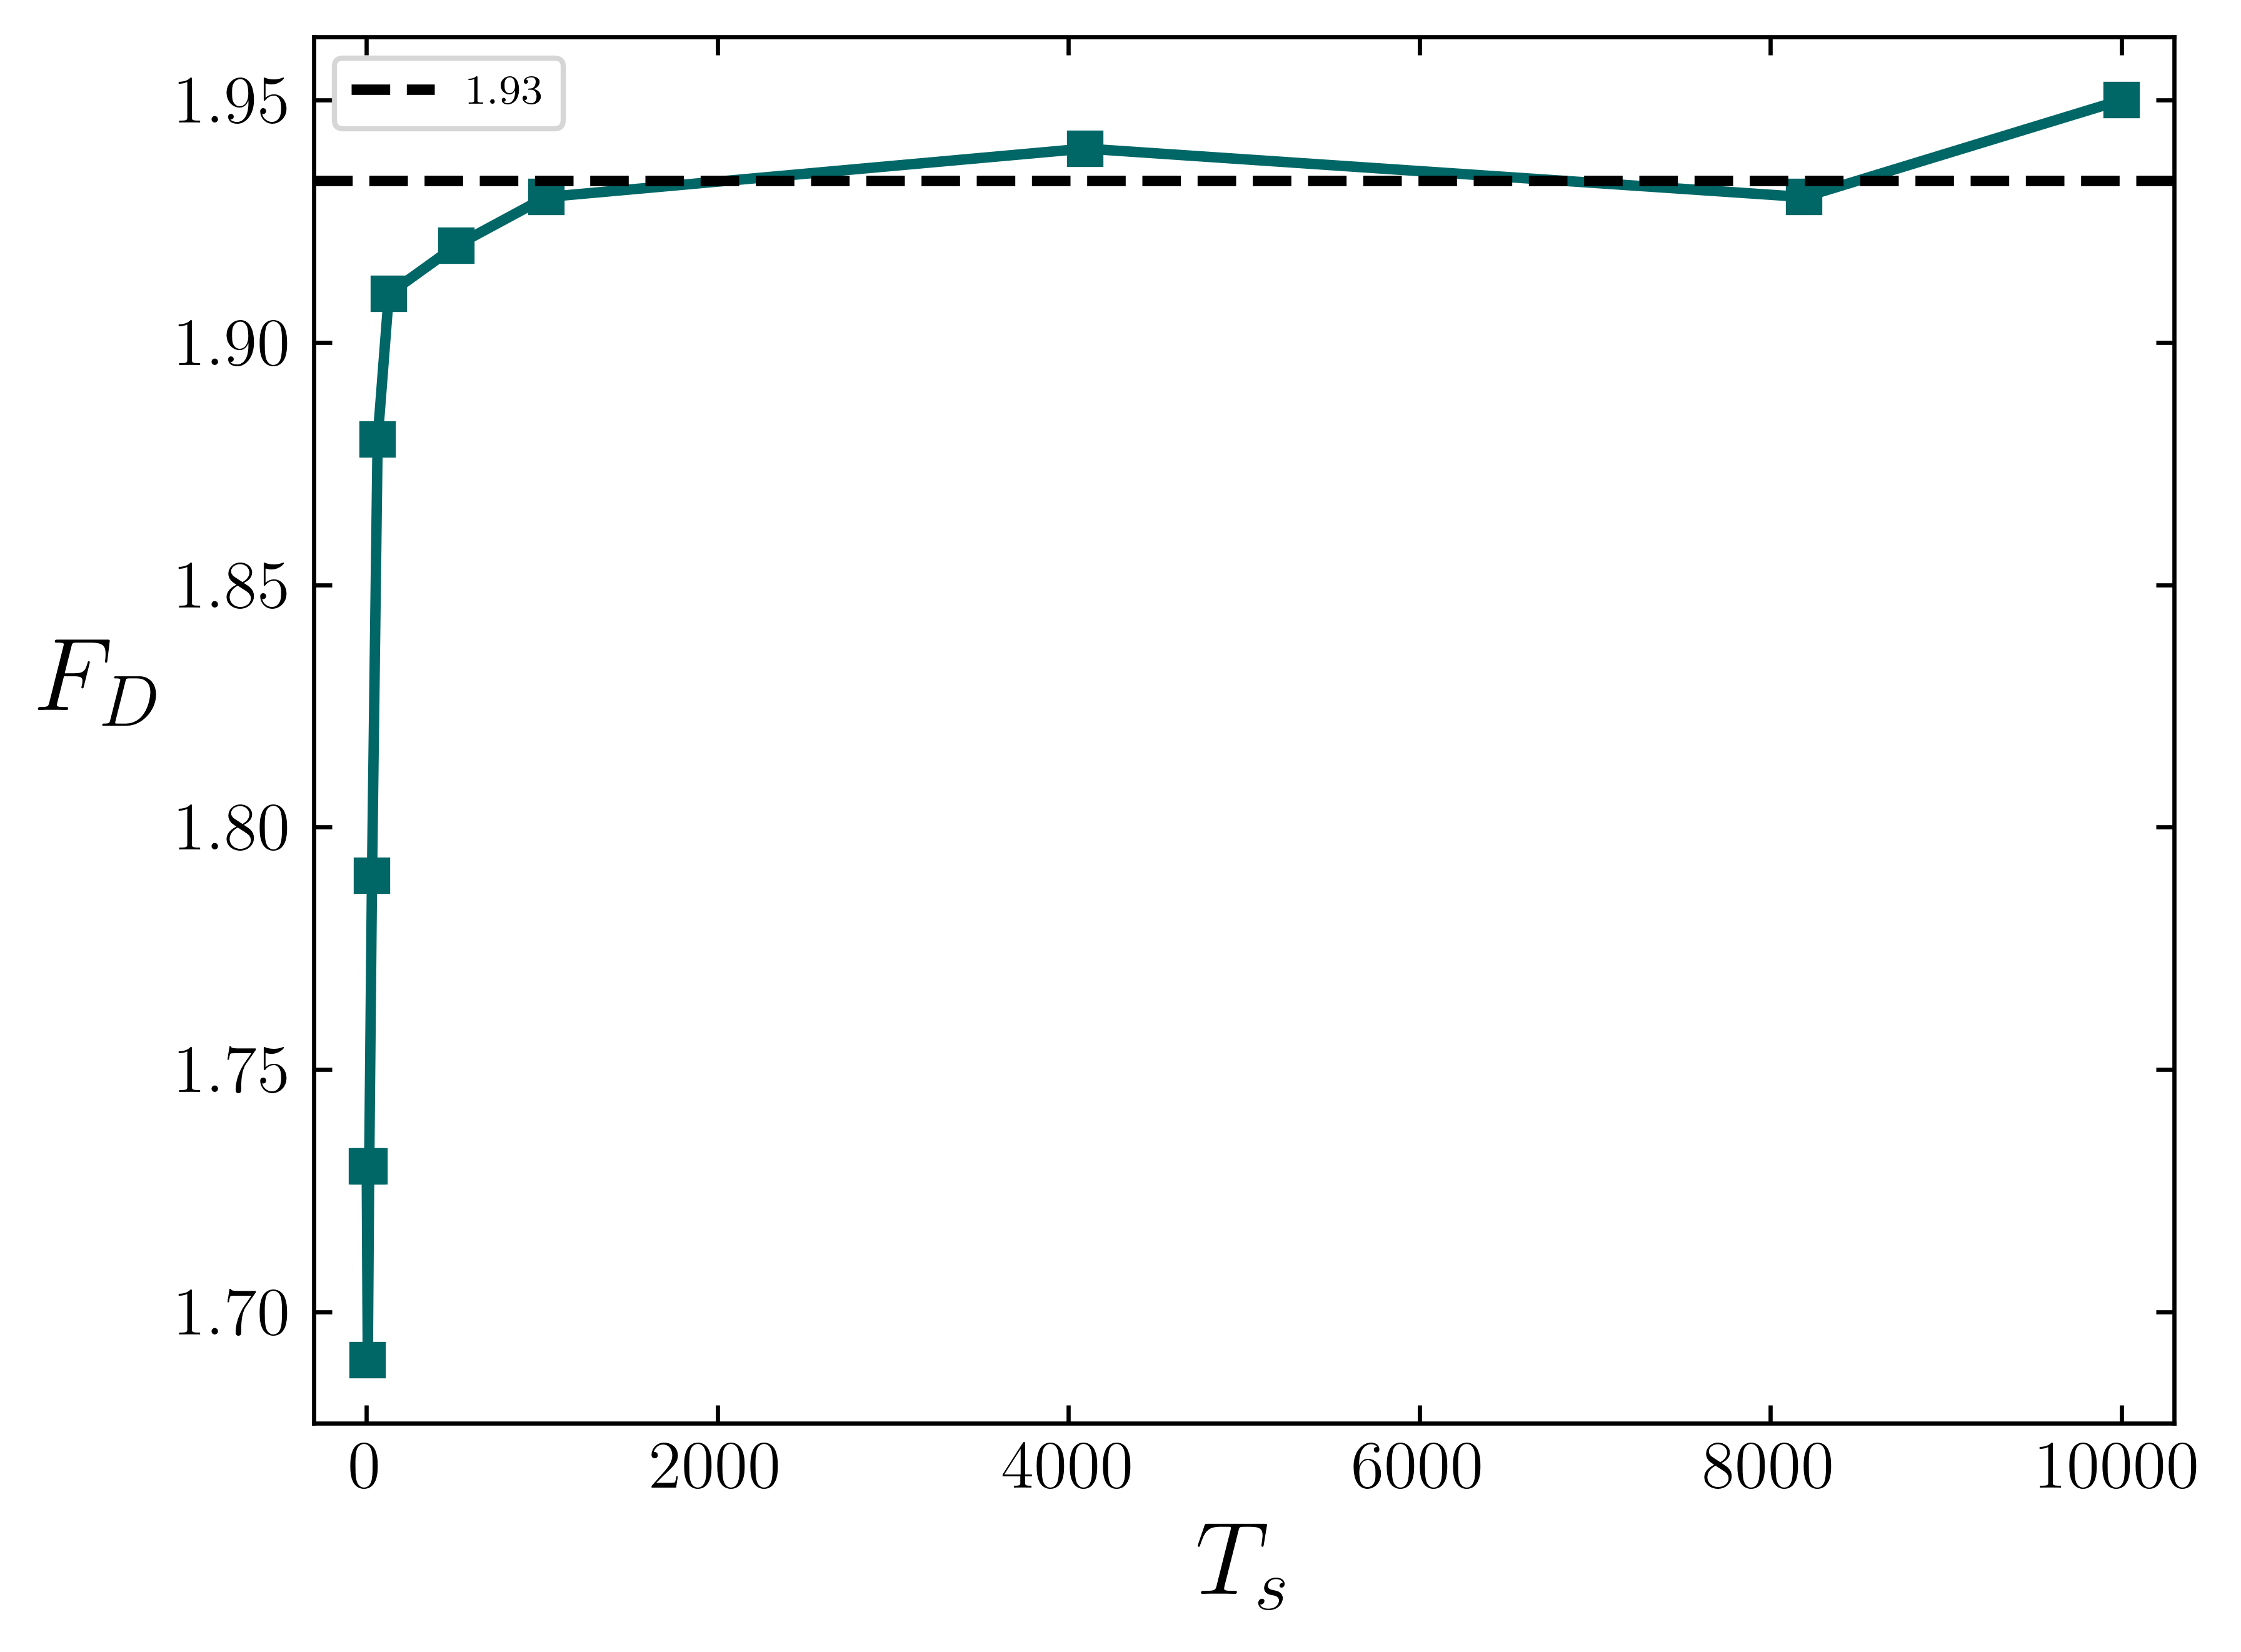
\includegraphics[width=\textwidth]{figures/dim_frac.png}

        \caption{ Gráfico da dimenssão fractal média,\(F_{D}\), em função do parâmetro de difusão \(T_{s}\). Os valores para 
        dimensão fractal foram obtidos por meio da média sobre diferentes seções de uma mesma fibrila e sobre os agregados
        de mesmo  \(T_{s}\). Usamos a relação massa-raio para determinar essa propriedade. A linha pontilhada representa 
        o valor médio da dimensão fractal para os valores de \(T_{S}=512,1024,4096,8192,10000\).} 

        \label{R4}
    \end{figure}


    \subsection{Propriedades mecânicas}

    \indent Para compreender como nosso agregado responde à aplicação de uma força axial, avaliamos como o número de 
    moléculas na fibrila varia com a força. Na Figura \ref{R5}, apresentamos a curva de stress-strain para agregados 
    gerados com diferentes valores de \(T_{s}\). Observamos que o aumento desse parâmetro influencia no incremento da 
    tensão máxima de ruptura, além disso, a deformação sofrida por essas fibrilas começa a ocorrer apenas para valores 
    de tensão mais altos, em comparação a fibrilas de baixo \(T_{s}\). No entanto, a partir de \(T_{s} = 512\), esses 
    valores se tornam bastante próximos e as curvas começam a se sobrepor. Comumente, esperaríamos que essas curvas crescessem de forma mais abrupta até o valor
    máximo, o que não é observado aqui. Esse comportamento mais suave até o valor limite é uma consequência do módulo 
    de Weibull que utilizamos no modelo. Para valores baixos, a curva resultante é não determinística 
    \cite{Parkinson1997}. A tensão máxima suportada que encontramos foi de 45,1 MPa, valor muito próximo ao encontrado 
    por Yang et al. \cite{YANG2012148} ao analisar fibrilas reconstituídas do tendão de Aquiles bovino purificado. 
    Em contraste, no trabalho de Yamamoto \cite{Noritaka}, foram utilizadas fibrilas isoladas do fascículo dos tendões 
    da cauda de ratos, obtendo um valor de 100 \(\pm\) 32 MPa. A discrepância em relação ao nosso valor pode estar 
    associada à dimensão das fibrilas utilizadas por ele, que apresentavam um diâmetro significativamente maior do que 
    as modeladas neste trabalho.

    \begin{figure}[H]
        \centering
        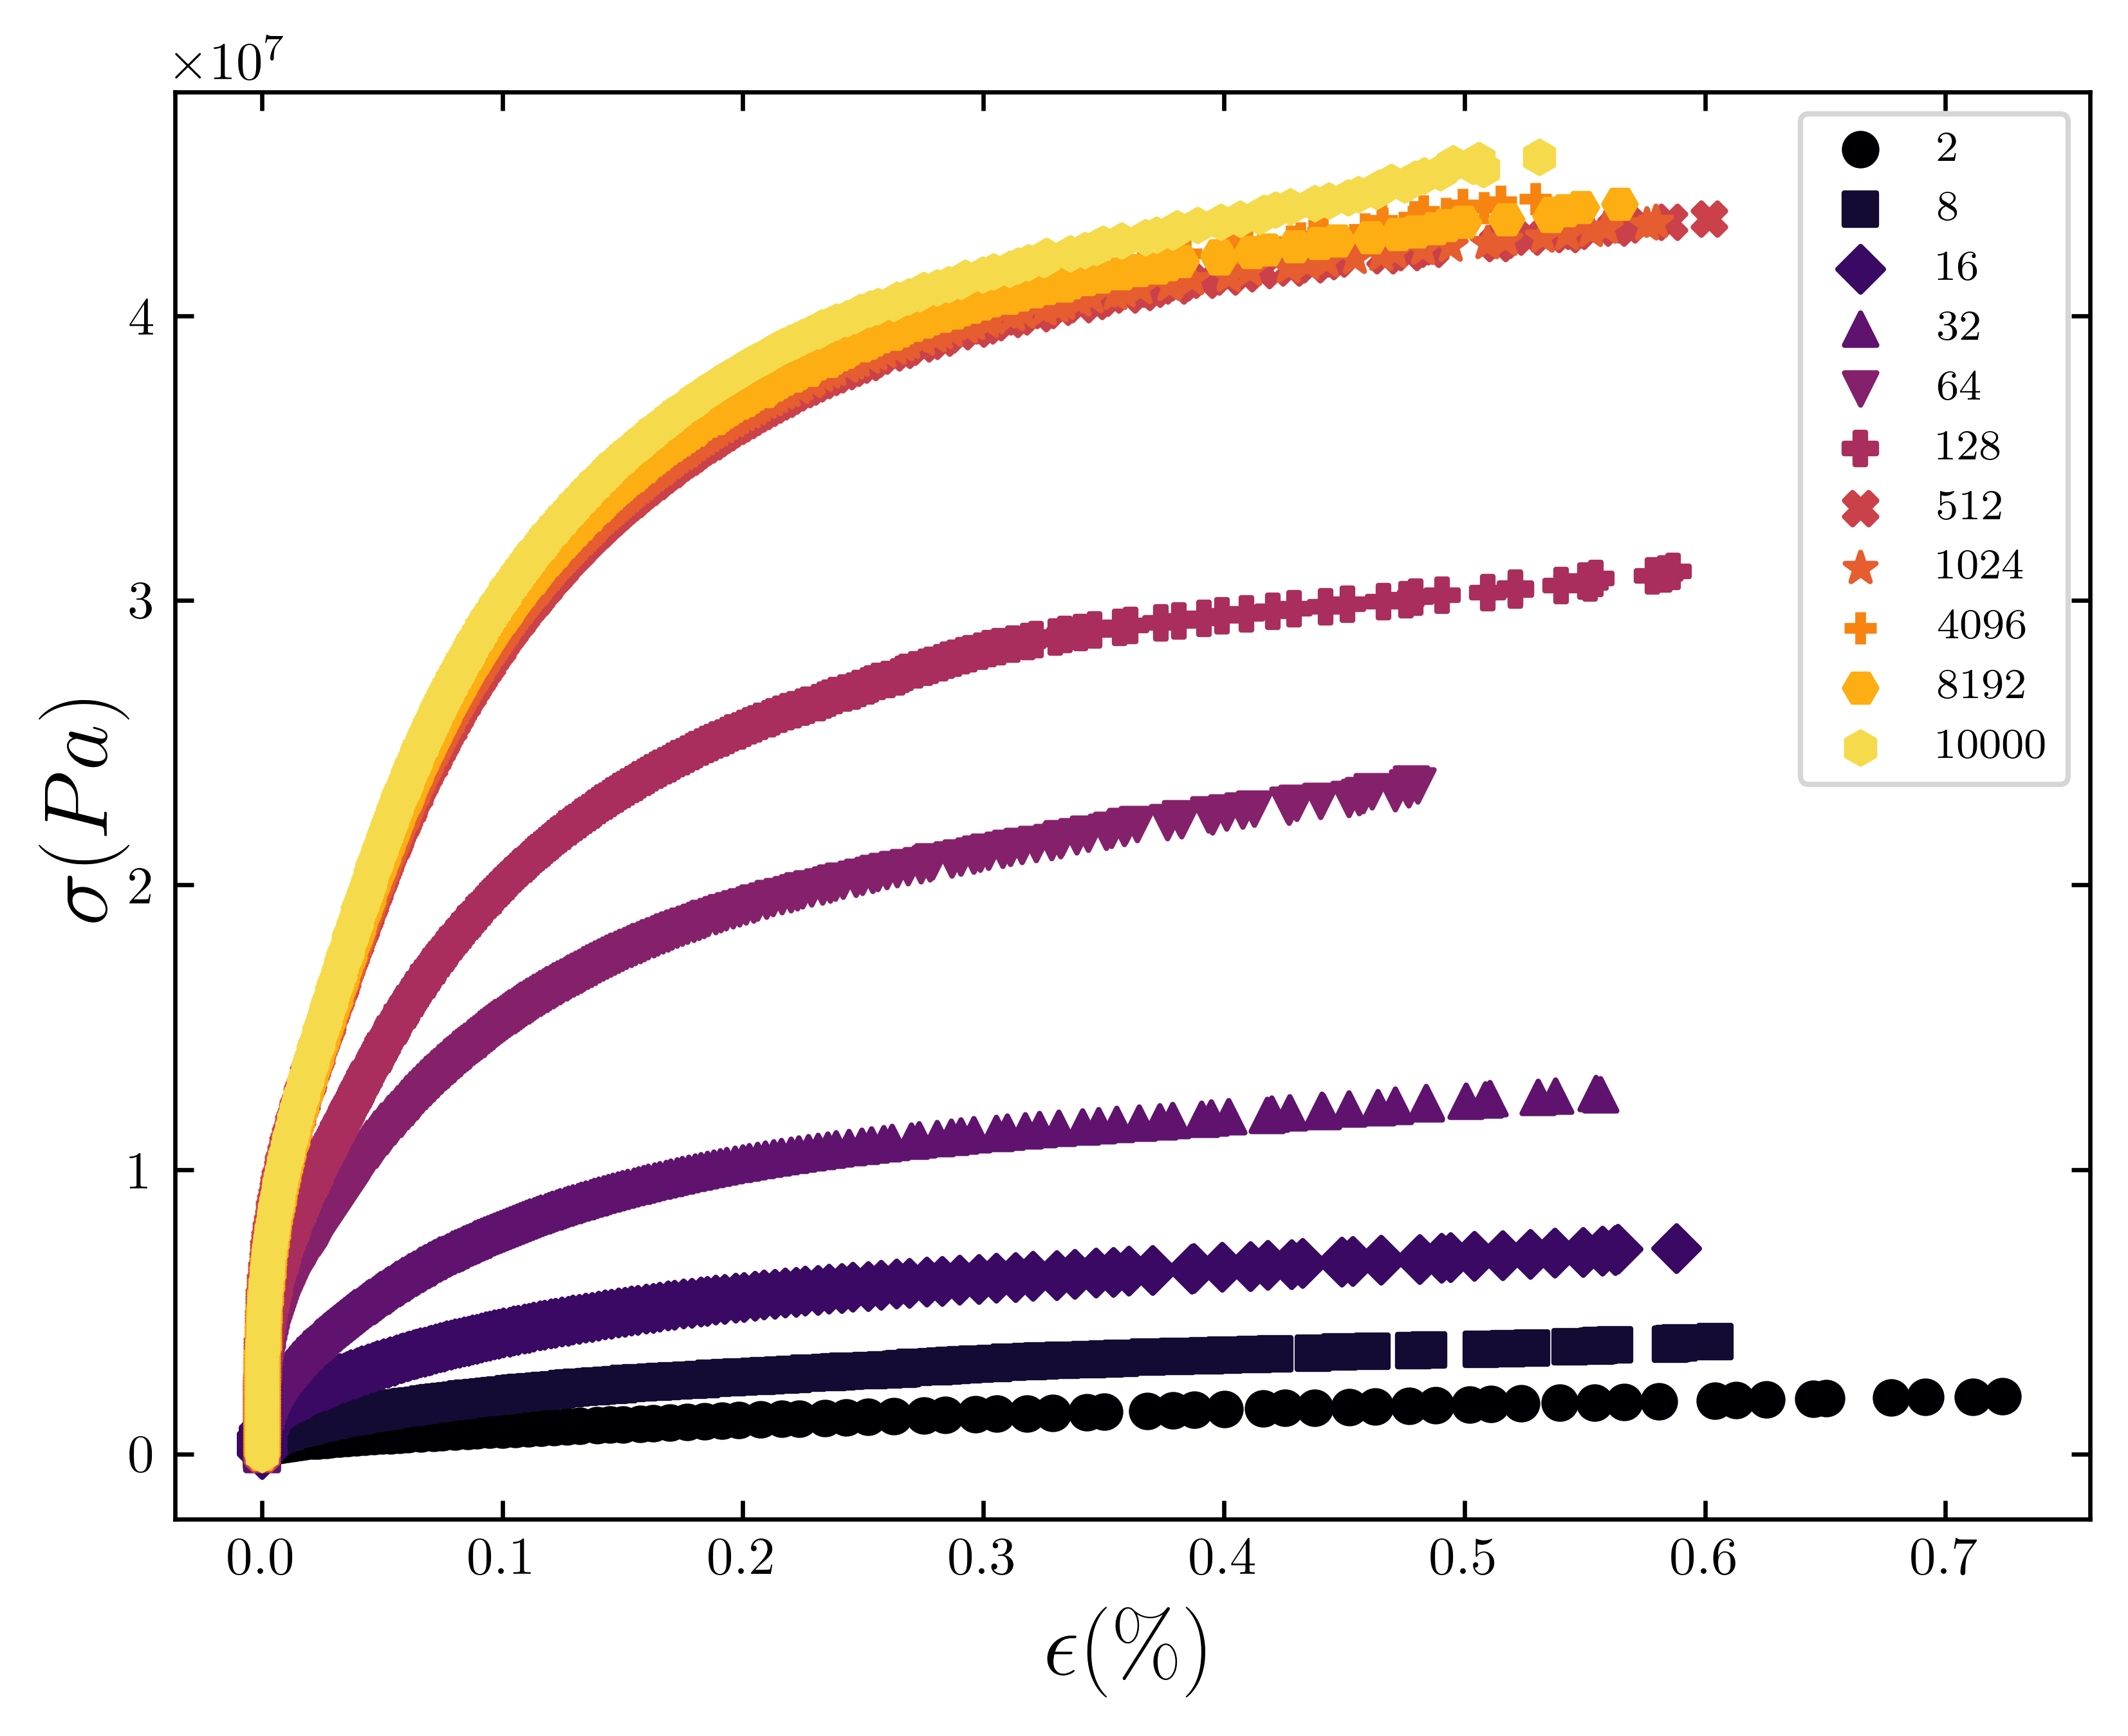
\includegraphics[width=\textwidth]{figures/stress_strain.png}

        \caption{Tensão em função da deformação da fibrila para diferentes valores de \(T_{s}\). A deformação foi calculada
        como a porção de moléculas removidas sobre o total de moléculas no inicio da simulação. Nos aproximamos a simualção 
        de uma medida real considerando que a unidade de força para romper as ligações internas equivale a  \( F_{c} = 0.5 nN\).} 

        \label{R5}
    \end{figure}

    Investigando o comportamento tensão em função da deformação, conseguimos determinar a existencia de dois regimes 
    para cada curva após elas começarem a sofrer deformação. Na Figura \ref{R8}, temos os comportamentos analisados para 
    as curvas de \(T_{s} = 8, 128, 1000\). Na região cinza, temos o comportamento não linear, regido por um logartimo 
    natural da forma \(A\times ln(BX)\). A separação ocorre proximo a \(28 \%\) de deformação das fibrilas. Após isso, 
    entramos em um regime linear, na região branca, da forma \(AX + B\). Na Tabela \ref{tab2}, temos os valores dos coeficientes
    das regressões para os dois regimes em cada parametro \(T_{s}\) e o \(R^{2}\). Novamente, para os valores a partir de \(T_{s} = 512\)
    , as curvas apresentam os coeficientes muito proximos, indicando que elas representam o mesmo processo de ruptura.

    \begin{figure}[H]
        \centering
        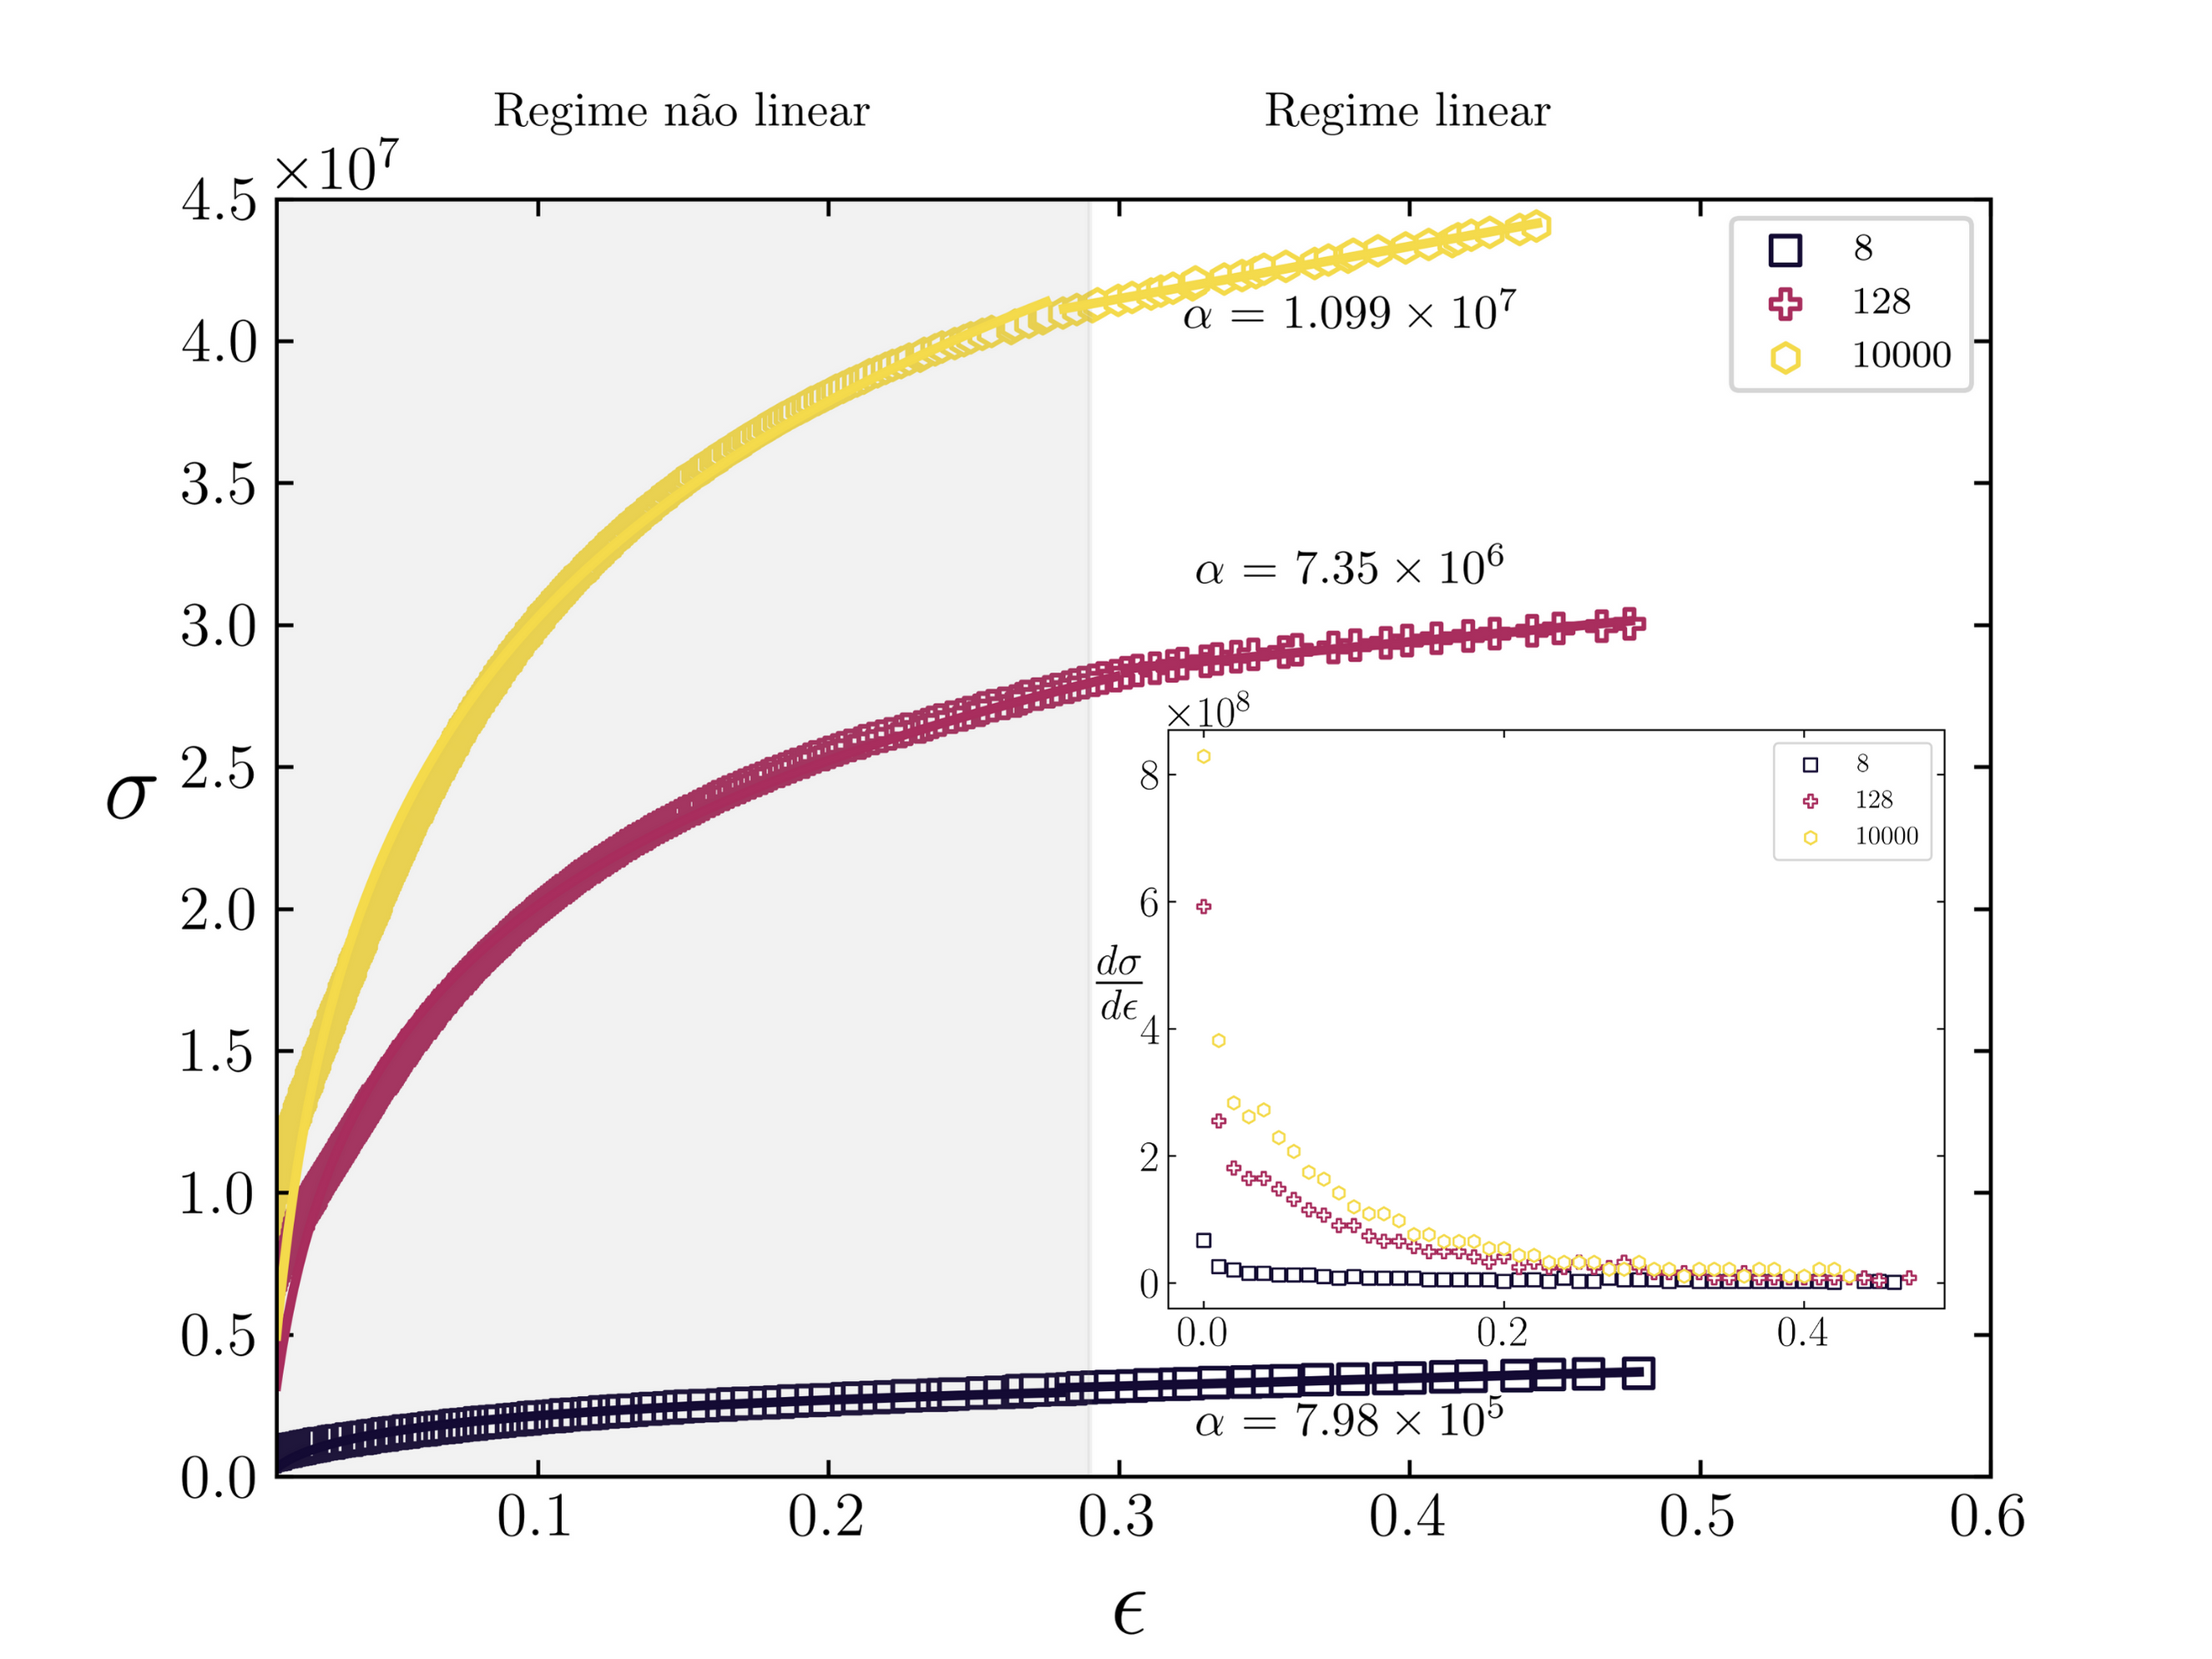
\includegraphics[width=\textwidth]{figures/stress_fit.png}

        \caption{Curva de tensão em função da deformação para \(T_{s} = 8, 128, 1000\). A região cinza delimita a 
        região de comportamento não linear. A região branca, o regime linear das curvas. O coeficiente angular de cada 
        curva é indicado. Na figura menor, temos o comportamento da derivada de cada curva de tensão, em função da 
        deformação.} 

        \label{R8}
    \end{figure}


    \begin{table}[H]
        \begin{tabular}{ccccl}
        \caption{Regressões para os diferentes regimes da curva de tensão deformação para os diferentes valores de \(T_{s}\).
        Os dois comportamentos, logaritmo natural e linear, estão acompanhados dos seus respectivos \(R^{2}\).}
        \hline
        \textbf{$T_{s}$} & \textbf{Aln(Bx)}                                                & \textbf{R\textasciicircum{}\{2\}} & \textbf{A + Bx}                                                                                              & R\textasciicircum{}\{2\} \\ \hline
        2                & 3.7 \textbackslash{}times 10\textasciicircum{}\{5\}ln(126.19x)  & 0.97                              & 8.98 \textbackslash{}times 10\textasciicircum{}\{5\} + 1.68 \textbackslash{}times 10\textasciicircum{}\{6\}x & 0.99                     \\
        8                & 7.98 \textbackslash{}times 10\textasciicircum{}\{5\}ln(146.69x) & 0.986                             & 2.34 \textbackslash{}times 10\textasciicircum{}\{6\} + 2.80 \textbackslash{}times 10\textasciicircum{}\{6\}x & 0.988                    \\
        16               & 1.65 \textbackslash{}times 10\textasciicircum{}\{6\}ln(140.8x)  & 0.988                             & 4.99 \textbackslash{}times 10\textasciicircum{}\{6\} + 3.95 \textbackslash{}times 10\textasciicircum{}\{6\}x & 0.998                    \\
        32               & 2.98 \textbackslash{}times 10\textasciicircum{}\{6\}ln(155.47x) & 0.99                              & 9.5 \textbackslash{}times 10\textasciicircum{}\{6\} + 5.86 \textbackslash{}times 10\textasciicircum{}\{6\}x  & 0.998                    \\
        64               & 5.7 \textbackslash{}times 10\textasciicircum{}\{6\}ln(145.58x)  & 0.989                             & 1.62 \textbackslash{}times 10\textasciicircum{}\{7\} + 1.60 \textbackslash{}times 10\textasciicircum{}\{7\}x & 0.997                    \\
        128              & 7.35 \textbackslash{}times 10\textasciicircum{}\{6\}ln(154.32x) & 0.99                              & 2.55 \textbackslash{}times 10\textasciicircum{}\{7\} + 9.37 \textbackslash{}times 10\textasciicircum{}\{6\}x & 0.99                     \\
        512              & 1.03 \textbackslash{}times 10\textasciicircum{}\{7\}ln(164.02x) & 0.99                              & 3.49 \textbackslash{}times 10\textasciicircum{}\{7\} + 1.6 \textbackslash{}times 10\textasciicircum{}\{6\}x  & 0.993                    \\
        1024             & 1.04 \textbackslash{}times 10\textasciicircum{}\{7\}ln(158.23x) & 0.99                              & 3.51 \textbackslash{}times 10\textasciicircum{}\{7\} + 1.58 \textbackslash{}times 10\textasciicircum{}\{7\}x & 0.99                     \\
        4096             & 1.08 \textbackslash{}times 10\textasciicircum{}\{7\}ln(157.09x) & 0.99                              & 3.65 \textbackslash{}times 10\textasciicircum{}\{7\} + 1.45 \textbackslash{}times 10\textasciicircum{}\{7\}x & 0.996                    \\
        8192             & 1.07 \textbackslash{}times 10\textasciicircum{}\{7\}ln(157.16x) & 0.991                             & 3.54 \textbackslash{}times 10\textasciicircum{}\{7\} + 1.7 \textbackslash{}times 10\textasciicircum{}\{7\}x  & 0.994                    \\
        10000            & 1.1 \textbackslash{}times 10\textasciicircum{}\{7\}ln(157.02x)  & 0.99                              & 3.59 \textbackslash{}times 10\textasciicircum{}\{7\} + 1.84 \textbackslash{}times 10\textasciicircum{}\{7\}x & 0.997                    \\ \hline
        \end{tabular}
        \label{tab2}
    \end{table}


    Na Figura \ref{R6}, podemos observar como os valores de tensão máxima suportada variam com um parâmetro 
    importante das fibrilas, a densidade. Escolhemos essa análise visto que o comportamento de \(\sigma\) e da 
    densidade, \(\rho\), exibem formas semelhantes quando analisados em função de \(T_{s}\). Identificamos um 
    comportamento exponencial no aumento da tensão máxima até um limite superior de 44,1 MPa. A saturação da 
    densidade ocorre em 65\%, valor este próximo ao encontrado por Parkinson et al.\cite{Parkinson1995} com esse 
    modelo, porém um pouco abaixo do determinado por Katz et al.\cite{KATZ1973351}, que calculou experimentalmente 
    cerca de 80\% do espaço disponível ocupado para as fibrilas de colágeno. Com base nessa característica de 
    saturação, consideramos que, dado o custo computacional elevado, este modelo pode ser executado, para os parâmetros 
    que inicialmente utilizamos, com \(T_{s}=512\), uma vez que nesse ponto já obtemos fibrilas com os valores de 
    interesse médios equivalentes para valores superiores desse parâmetro. 



    \begin{figure}[H]
        \centering
        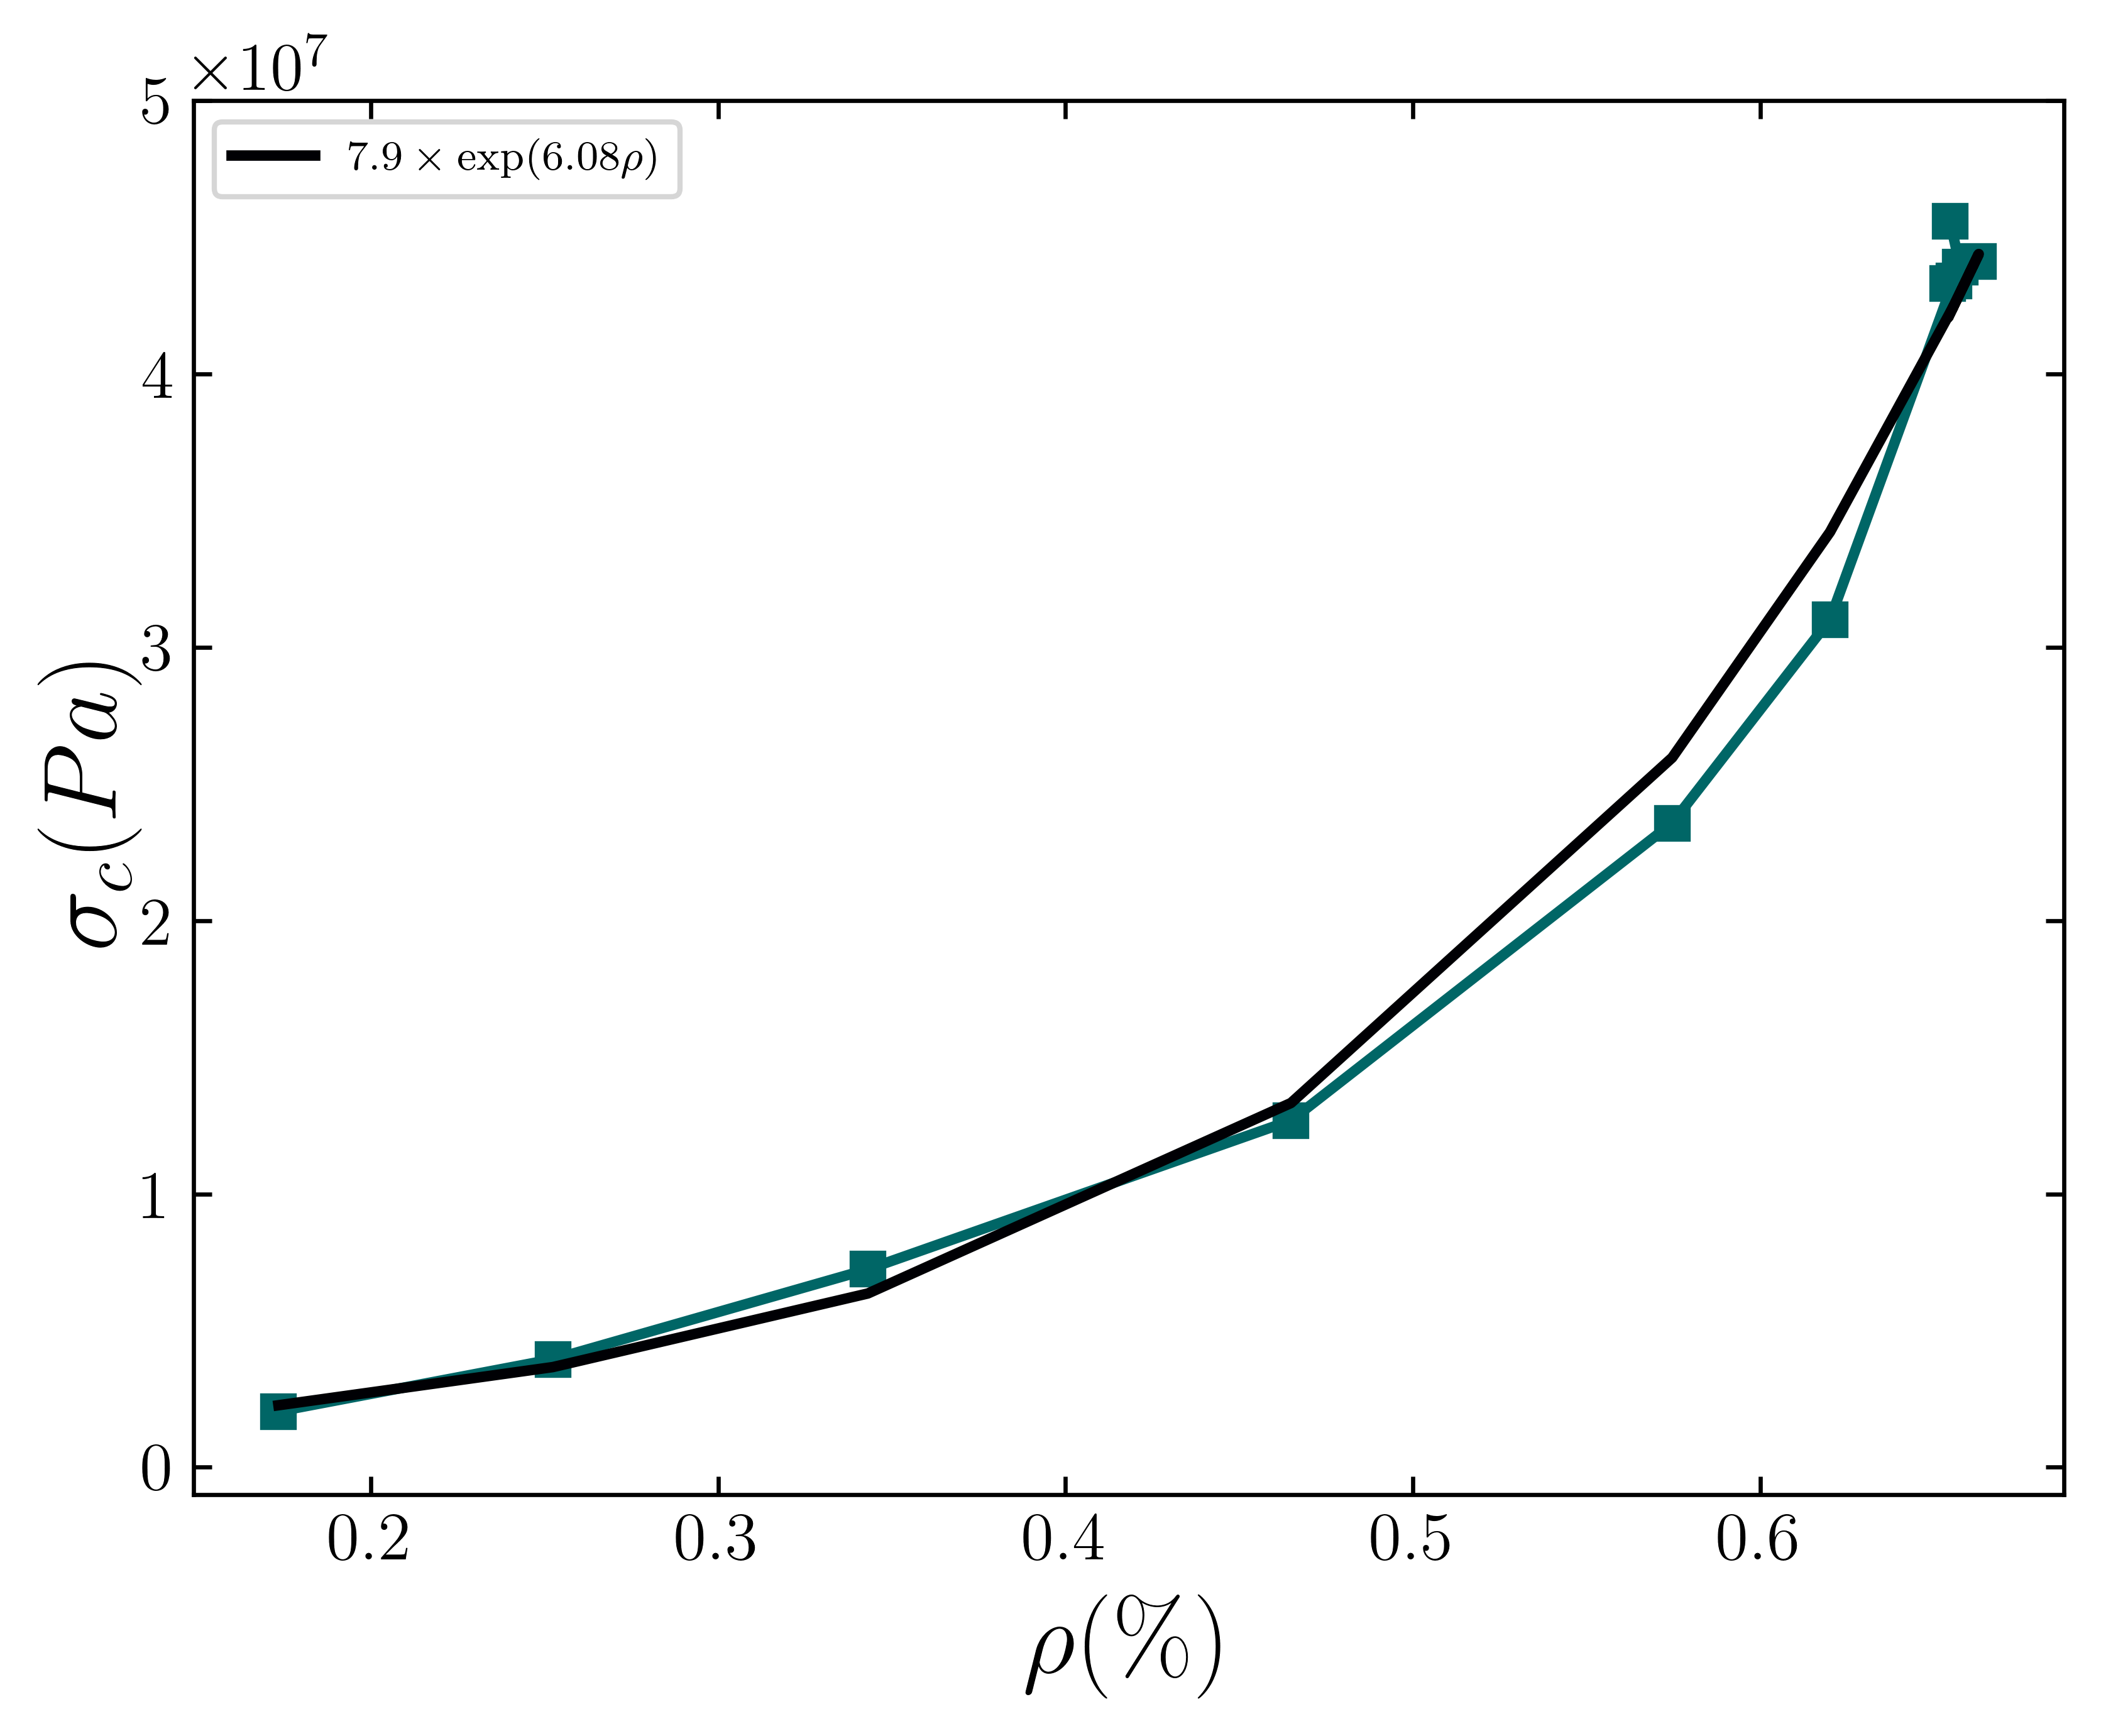
\includegraphics[width=\textwidth]{figures/sigma_rho.png}

        \caption{Tensão crítica em função da densidade das fibrilas. Os dados medidos são os quadrados verdes. A curva 
        continua preta é o ajuste exponencial dos dados. A forma da exponencial, mostrada na legenda da curva, é dada 
        por \(6.95 \times 10^{5}e^{6.08\rho}\).} 


        \label{R6}
    \end{figure}

    Ao analisar como o processo de ruptura ocorre no nosso modelo, bem como em outros, constatamos que a 
    redistribuição de tensão, para uma mesma força, pode levar à ocorrência de rupturas em cascata. Na Figura 
    \ref{R7}, apresentamos a distribuição das avalanches de ruptura em função do seu tamanho. É possível observar a 
    existência de duas ordens de grandeza bem definidas; após isso, os dados são afetados pelo efeito de tamanho 
    finito. Analisando a região de interesse, até próximo de \(10^{2.5}\), conseguimos determinar o expoente das leis 
    de escala de modo que eles aumentam com o crescimento de \(T_{s}\). Este comportamento é compreensível ao 
    considerarmos que a densidade aumenta com este parâmetro, resultando em mais moléculas para contribuir com os 
    tamanhos das avalanches. Assim, temos que as avalanches durante o processo de ruptura são independentes do tamanho 
    do sistema; contudo, elas são influenciadas pelo quão compacta é a fibrila, com o expoente \(\gamma\) variando de 
    -1.94 até -2.60. Na Tabela \ref{tab3}, temos os outros coeficientes para cada valor do parâmetro \(T_{s}\).
    


    \begin{figure}[H]
        \centering
        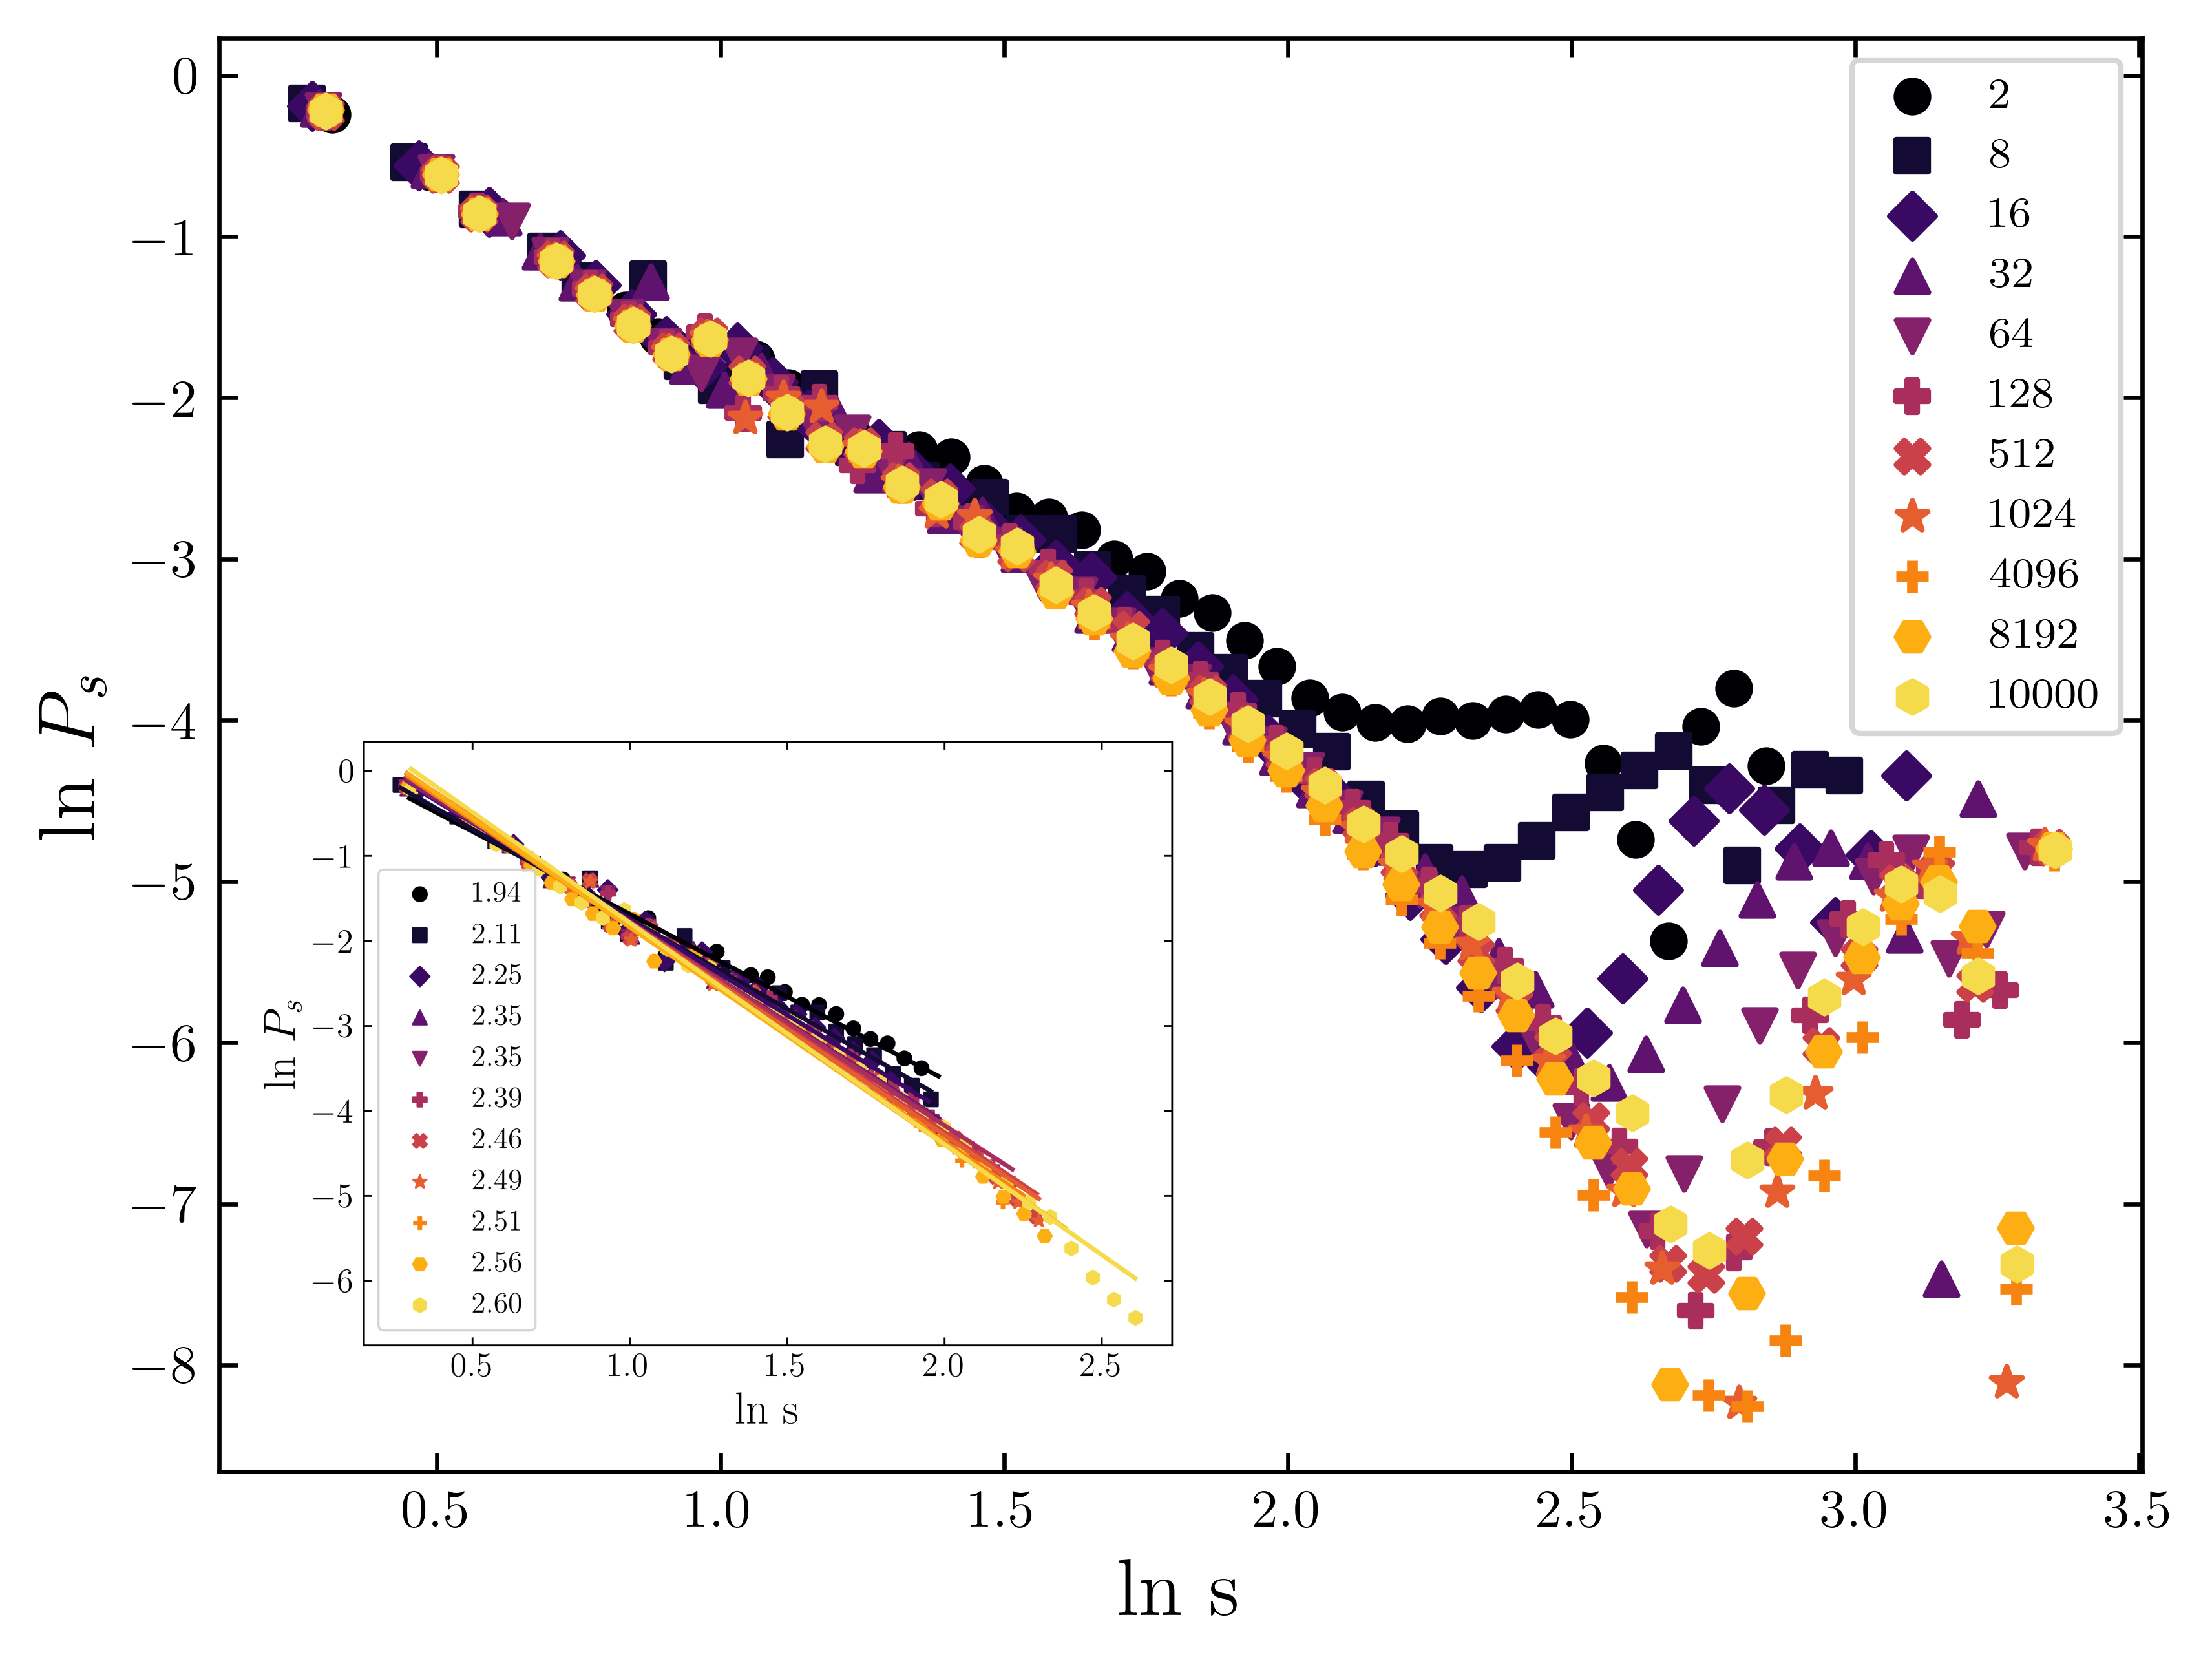
\includegraphics[width=\textwidth]{figures/ava.png}

        \caption{Distribuição das avalanches de ruptura em função do seu tamanho para diferentes valores de \(T_{s}\).
        Podemos observar um comportamento em lei de potencia com expoentes $\gamma$ bem definidos para todos valores do 
        parâmetro. Os expoentes variam de -1.94 a -2.60.} 

        \label{R7}

    \end{figure}

    \begin{table}[H]
        \begin{tabular}{cc}
        \caption{Expoente \(gamma\) das leis de escala das avalanches para cada parâmetro \(T_{s}\).}
        \hline
        \textbf{\(T_{s}\)} & \textbf{\(gamma\)} \\ \hline
        2                  & 1.94               \\
        8                  & 2.11               \\
        16                 & 2.25               \\
        32                 & 2.35               \\
        64                 & 2.35               \\
        128                & 2.39               \\
        512                & 2.46               \\
        1024               & 2.49               \\
        4096               & 2.51               \\
        8192               & 2.56               \\
        10000              & 2.6                \\ \hline
        \end{tabular}
        \label{tab3}
    \end{table}

\section{Conclusões}

    Neste estudo, demonstramos a capacidade de um modelo baseado em Agregação Limitada por Difusão (DLA) com difusão 
    superficial para simular a formação de fibrilas de colágeno, resultando em agregados com características morfológicas 
    semelhantes às das fibrilas reais. O parâmetro \(T_{s}\) mostrou-se cruciail para definir várias propriedades das 
    fibrilas, como comprimento, densidade e diâmetro, que tendem a variar de maneira inversamente proporcional a \(T_{s}\). 
    Observou-se uma relação linear entre a massa das fibrilas e a distância até as pontas, além de uma variação na dimensão 
    fractal da seção central, que aumenta com \(T_{s}\), variando de 1.71 a 1.93.

    A resistência máxima à tensão das fibrilas aumenta com \(T_{s}\), alcançando um limite de 44,1 MPa, e a tensão crítica 
    suportada apresenta uma correlação exponencial com a densidade das fibrilas. O processo de ruptura revelou avalanches 
    de ruptura com leis de potência definidas, cujos expoentes variam de -1.94 a -2.60, indicando que, embora as avalanches 
    sejam independentes do tamanho do sistema, elas são influenciadas pela compactação da fibrila.

    Essas descobertas sugerem que as fibrilas geradas pelo modelo apresentam uma tensão máxima suportada que aumenta com a 
    densidade e com \(T_{s}\). Fibrilas mais resistentes tendem a ter uma dimensão fractal mais próxima da dimensão 
    euclidiana de objetos bidimensionais e exibem valores mais elevados no expoente das leis de potência. Além disso, muitas 
    das propriedades analisadas tendem a saturar, indicando que simulações realizadas com \(T_{s} = 512\) são suficientes para 
    observar os valores máximos de interesse, otimizando o uso de recursos computacionais.


\bibliographystyle{unsrtnat} % Ou outro estilo de sua preferência
\bibliography{ref} % Refere-se ao seu arquivo ref.bib, sem a extensão .bib


    
\end{document}
